\chapter{Implementation and Experimental Results}
\label{chapter_Experimental_Results}

This Chapter is dedicated to describe the experimental validation of the methodology presented in the previous Chapter. Extensive results and analysis are presented to explore each of the steps in the proposed methodology. In particular, we focus on both the robustness of the domain characterization and in the accuracy of the results obtained from the spatio--temporal predictive queries. In each case, we employ alternative methods as baseline for comparing the performance of the proposed approach.

Several aspects of the methodology have been implemented in the form of a software called ``Spatio-Temporal Tool for Time Series Analysis'' or SPT-TSA. This software is the subject of the next section.

\section{Spatio Temporal Framework for Time Series Analysis}       
\label{Sec:SPTA-TSA}

We will describe the architectural design of SPT-TSA, a Python 3 package built to work with spatio-temporal data and predictive models. This package was developed as an implementation of a computational solution to execute the methodology described in the previous Chapter, but it can be extended to be used for other similar purposes in the field of spatio-temporal analysis.

\subsection{SPTA-TSA Workflow}
\label{Sec:SPTA-TSA_Workflow}

When dealing with spatio-temporal data and in particular time series data, it is possible to find libraries and packages to perform operations for data manipulation and time series analysis, particularly in the Python and R programming languages. Our software SPTA-TSA was designed to leverage widely known libraries and packages developed for Python 3, such as pandas \cite{McKinney2010}, scikit-Learn \cite{scikit-learn2011}, tslearn \cite{tslearn2020}, Keras \cite{Chollet2015}, TensorFlow \cite{tensorflow2016}, pickle, NumPy \cite{Harris2020}, MatplotLib, among others.
t
\begin{figure}[tp]
	%\begin{minipage}[b]{0.8\textwidth}
	\centering
	\includegraphics[scale=0.25, angle=90]{../Figures/workflow_data_operations}
	\caption{Steps for Dataset Transformation and Generated Products.}	
	\label{Fig:Steps-Data-Transformation}	 		
\end{figure}

Figure \ref{Fig:Steps-Data-Transformation} shows the workflow operations made available by SPTA-TSA, as well as the libraries and packages responsible for the manipulation and analysis of spatio-temporal data. Each color represents the following:

\begin{description}
    \item[In Blue:] Library dependencies and packages required for the operations, focusing on manipulation of time series data and time series analysis .
    \item[In Red:] The name of the operations performed, these can be matched with important tasks required by the methodology proposed in the previous chapter.
    \item[In Black:] The name of the attributes of the dataset and the options available in the implementation to perform each operation.
    \item[In Green:] The output products in each operation in the form of a file (CSV, graphic, serial or NPY).
\end{description}

The rest of the section describe the Class diagrams that captures the logical structure of the SPTA-TSA implementation.

\subsection{Class Diagrams}
\label{Sec:SPT-TSAClassDiagrams}

To better describe the functionality and architectural design of SPT-TSA, we present two class diagrams, each showing a different, noteworthy aspect of the implementation. Figure \ref{Fig:DiagramClasess-Region} shows a class diagram concerning the implementation of spatio-temporal regions and operations that can be applied to them. The diagram indicates that spatio-temporal and spatial regions are built upon a common domain region, on which operations can be performed. The operations are special functions (hereby called function regions) that can be applied to either spatial or spatio-temporal regions, and can produce them as output. This means that, in SPT-TSA, these operations are transformations of domain regions. Additional properties of spatio-temporal regions, such as grouping from partitioning schemes and the scaling of temporal data, are achieved using decorators.

\begin{figure}[tp]
	%\begin{minipage}[b]{0.8\textwidth}
	\centering
	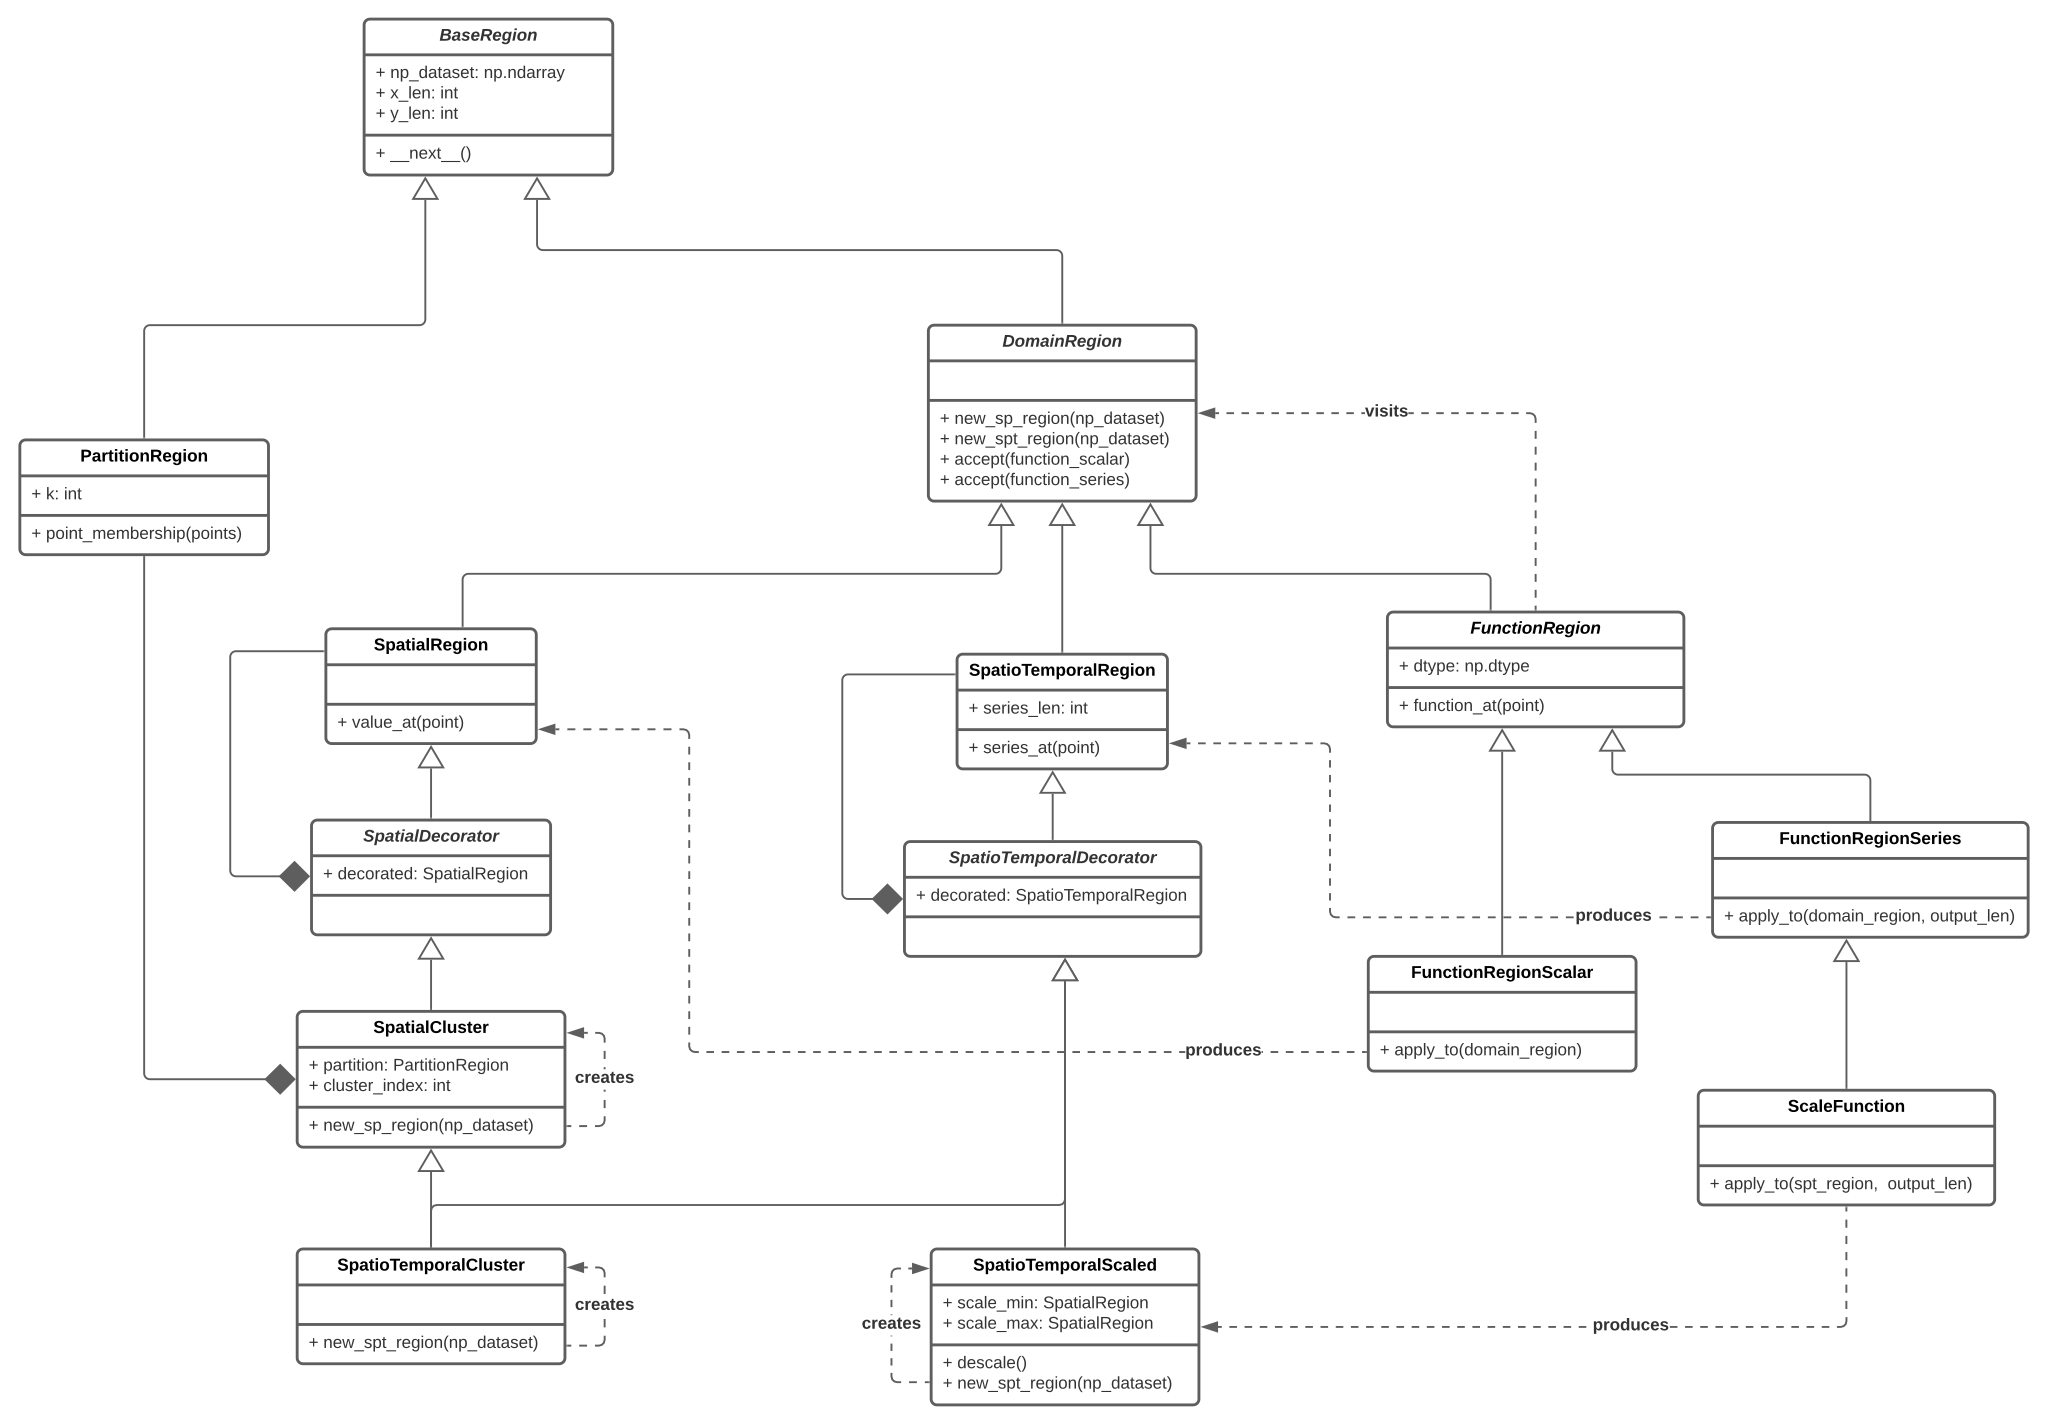
\includegraphics[scale=0.41, angle=90]{../Figures/SPT-TSA-RegionClasses}
	\caption{Class Diagram -- Region Class.}	
	\label{Fig:DiagramClasess-Region}	 		
\end{figure}

A brief description of each class is provided:

\begin{itemize}
	\item \texttt{Point}: a simple implementation of a 2D position with $(x, y)$ coordinates.
	
	\item \texttt{BaseRegion}: The base class for all regions. It is a wrapper of a \texttt{numpy.ndarray} object, which constrains the dimensions of the region inside a 2D rectangle. In addition to providing basic functions such as saving a dataset to persistent storage, it allows the iteration of the domain points contained within the 2D boundary, using Point instances.
	
	\item \texttt{PartitionRegion}: Describes the application of a partitioning scheme to divide a spatio-temporal region into groups, by storing the membership of each point in the region to a group. Note that it is kept separate from \texttt{DomainRegion}, because it is not meant to accept function regions.
	
	\item \texttt{DomainRegion}: The parent class of both spatial and spatio-temporal regions, and also the operand and result of function regions. This abstract implementation has common functionalities for both 2D and 3D arrays, and can be used to create new spatial and spatio-temporal regions that are of a particular instance. Since function regions transform a domain region into a new region, we allow subclasses to determine which new instance to create by leveraging polymorphism. For example, a function region acting on an instance of \texttt{SpatialRegion} may produce a new \texttt{SpatialRegion} instance using the \texttt{new\_sp\_region} method declared in this class. However, that same function region acting on an instance of \texttt{SpatialCluster}, using the same \texttt{new\_sp\_region} method, will produce an instance of \texttt{SpatialCluster} instead, due to the polymorphic method call. 
	
	\item \texttt{SpatialRegion}: The 2D implementation of \texttt{DomainRegion}, it stores a value in each point. Iterations of the points in the domain will yield the values for each point.
	
	\item \texttt{SpatioTemporalRegion}: The 3D implementation of \texttt{DomainRegion}, it stores an array in each point, representing a time series. Iterations of the points in the domain will yield the series for each point.
	
	\item \texttt{FunctionRegion}: A special type of \texttt{DomainRegion} used to transform \texttt{DomainRegion} instances, by accepting a \texttt{DomainRegion} instance as input and producing another \texttt{DomainRegion} instance as output, potentially of a different type. It serves as a common class for \texttt{FunctionRegionScalar} (produces a \texttt{SpatialRegion} instance as output) and \texttt{FunctionRegionSeries} (produces a \texttt{SpatioTemporalRegion} instance as output). The transformation of the input is achieved by storing a Python function at each point of the function region, and applying each function to the corresponding element in the operand region. To represent this application, consider a spatial region $S_{(m,n)}$ and a function region $F_{(m,n)}$, we then have $F(S) = \left\{ f_{ij}(s_{ij}); (i, j) \in [0, m]\times[0, n] \right\}$. See \texttt{FunctionRegionScalar} for practical examples.
	
	The implementation uses the Visitor pattern, where the \texttt{DomainRegion} is the visitor that `visits' the function region to retrieve the corresponding function during an iteration of points. The benefit of the visitor approach is that the same \texttt{FunctionRegion} can be applied to different subclasses of \texttt{SpatialRegion} and \texttt{SpatioTemporalRegion} without knowledge of the particular subclasses, while still producing different and expected outputs. A limitation of this approach is that only one function region can be applied to a given region at any given time, otherwise the iterator of the region will be used twice and become corrupted.
	
	\item \texttt{FunctionRegionScalar}: A subclass of \texttt{FunctionRegion} that produces a subclass of \texttt{SpatialRegion} when applied to a \texttt{DomainRegion}, regardless of the input domain being spatial or spatio-temporal. The implementation will call the \texttt{new\_sp\_region} method of the operand polymorphically to produce the desired output.
	
	For an example, consider the problem of averaging each series in a spatio-temporal region, by using the function \texttt{numpy.mean} to the series at each point of the region. This can be achieved by creating an instance of \texttt{FunctionRegionScalar} so that each point of its internal 2D array contains the function \texttt{numpy.mean} itself, and applying this function region to the spatio-temporal region. 
	
	\item \texttt{FunctionRegionSeries}: Analogous to \texttt{FunctionRegionScalar} but will always produce a subclass of \texttt{SpatioTemporalRegion} by calling the \texttt{new\_spt\_region} method of the input. It requires to know the length of the output series in advance in order to allocate the output 3D array.
	
	\item \texttt{ScaleFunction}: A subclass of \texttt{FunctionRegionSeries} that produces an instance of \texttt{SpatioTemporalScaled} (see below) when applied to a \texttt{SpatioTemporalRegion}.
	
	\item \texttt{SpatialDecorator}: Implementation of the Decorator pattern for a \texttt{SpatialRegion}.
	
	\item \texttt{SpatialCluster}: A decorated version of \texttt{SpatialRegion} that provides support for describing clusters obtained from a partitioning scheme. Each instance of \texttt{SpatialCluster} represents one group only (a group index is used), so $k$ instances would be required to represent the output of a partitioning scheme of $k$ groups. Iterations of \texttt{SpatialCluster} will only yield the points that are members of the corresponding group, and attempts to read the value of a point outside the group result in error. This effect is achieved by keeping the same underlying data for all the $k$ instances (no additional copies are made), as well as the same instance of the  \texttt{PartitionRegion} but with a corresponding group index. The behavior is implemented by decorating the relevant methods in order to use the partition and the index.
	
	\item \texttt{SpatioTemporalDecorator}: Implementation of the Decorator pattern, but this time for a \texttt{SpatioTemporalRegion}.
	
	\item \texttt{SpatioTemporalCluster}: A decorated version of \texttt{SpatioTemporalRegion} that provides support for describing clusters obtained from a domain partitioning technique. This class uses multiple inheritance to also extend \texttt{SpatialCluster} in order to include cluster behavior, while at the same time working with a 3D array to store a series at each point.
	
	\item \texttt{SpatioTemporalScaled}: A decorated version of \texttt{SpatioTemporalRegion} that represents the scaled version of a spatio-temporal region. The scaling process is performed by a \texttt{ScalingFunction}, which will iterate each point to independently scale the corresponding series. A series is scaled by finding its minimum and maximum values so that the new values are in the $[0, 1]$ interval. These minimum and maximum values are stored as two \texttt{SpatialRegion} instances inside the scaled region, so that the original values can be restored at a later point. 
	
	Consider the example of partitioning a spatio-temporal region: this can be achieved b applying both the \texttt{SpatioTemporalCluster} and \texttt{SpatioTemporalScaled} decorators since it is possible to chain them. The expected output (a cluster representing a group of scaled series at each point) is obtained even if the decorators are applied in different order. Reverting the scaling will yield a \texttt{SpatioTemporalCluster} again.
\end{itemize}

The second class diagram is shown in Figure \ref{Fig:DiagramClasess-Models}. The main focus is now the analysis of the forecast error. Here, we find classes related to the training of predictive models, their forecasting of future values of the predictive variable, and the subsequent calculation of the forecast error when the actual values are available. The descriptions provided here are for the relevant ARIMA predictive models. Other predictive models used as baseline for comparison follow a similar class structure.

\begin{figure}[tp]
	%\begin{minipage}[b]{0.8\textwidth}
	\centering
	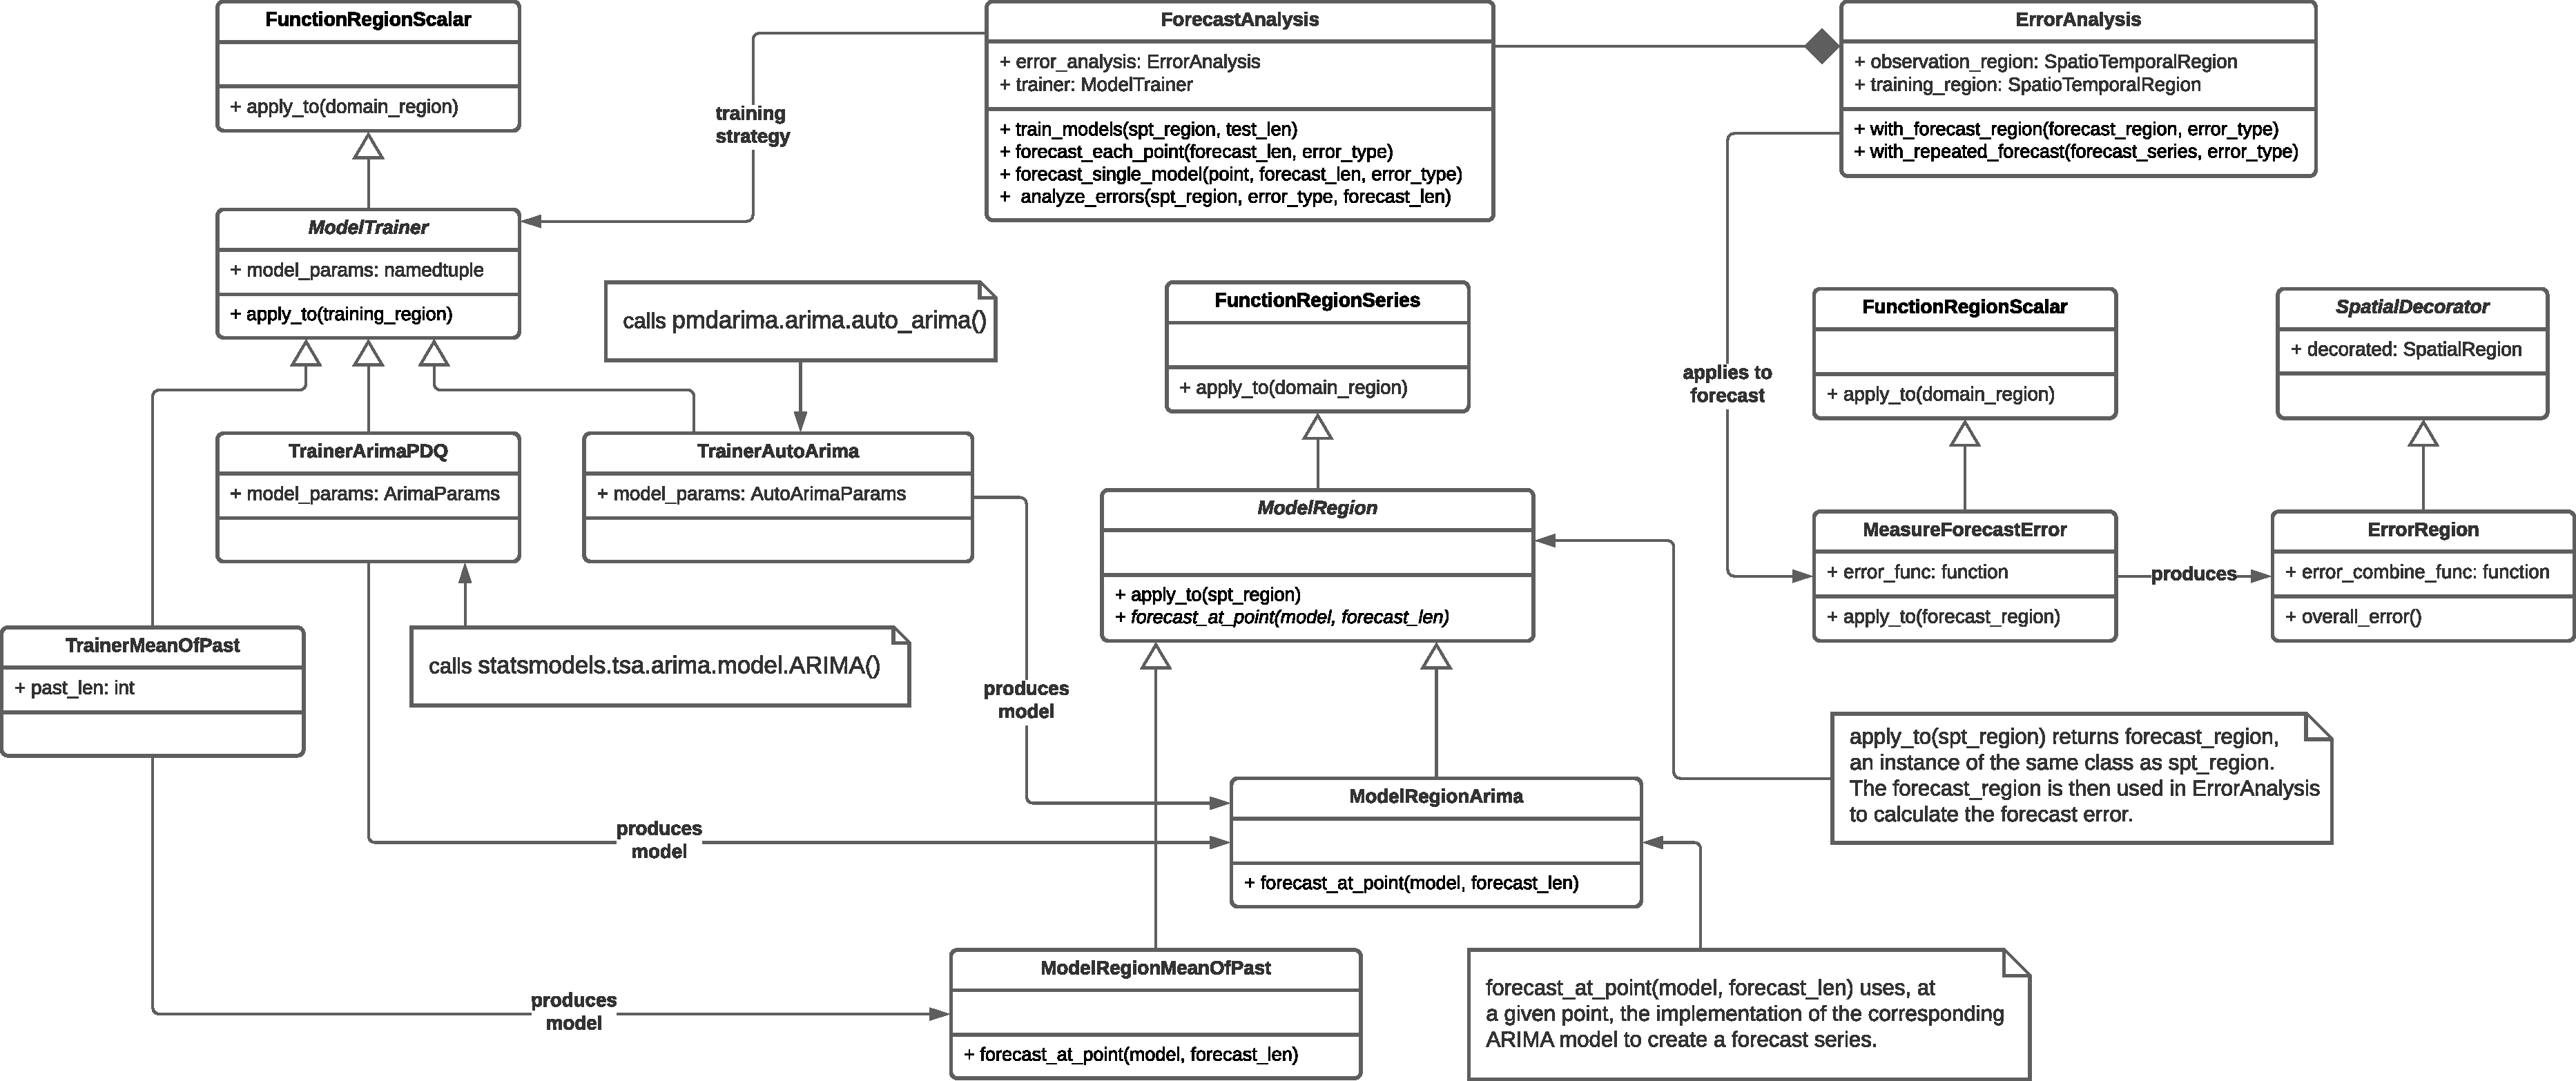
\includegraphics[scale=0.37, angle=90]{../Figures/SPT-TSA-ModelsClasses}
	\caption{Class Diagram -- Model Class.}	
	\label{Fig:DiagramClasess-Models}	 		
\end{figure}

\begin{itemize}
	\item \texttt{ModelRegion}: Base class for the different predictive models supported by SPT-TSA. A model will produce, for each point in a spatio-temporal region, a series that represents the predicted values of the predictive variable. This is achieved by extending the behavior of \texttt{FunctionRegionSeries}, where the length of the series represents to the size of the forecast. If, for example, we pass an instance of \texttt{SpatioTemporalRegionScaled} as an operand, then the output is also scaled, and the  original scaling information can be used to recover the desired forecast series.
	
	\item \texttt{ModelTrainer}: Base class for training predictive models supported by SPT-TSA. The models are trained by passing a training spatio-temporal region containing, for each point, a training series (same length for all points in the region). The implementation overrides the behavior of \texttt{FunctionRegionScalar} to produce an instance of \texttt{ModelRegion} instead of \texttt{SpatialRegion}. The exact class of the instance and its properties (resulting model parameters) will depend on the subclasses of \texttt{ModelTrainer} and how they process the \texttt{model\_params} input.
	
	\item \texttt{TrainerArimaPDQ}: A model trainer that will use, for each point, the class \\ \texttt{statsmodels.tsa.arima.model.ARIMA} to fit an ARIMA model using a training series and a $(p, d, q)$ tuple. The result of applying this function to a training region is an instance of \texttt{ModelRegionArima}.
	
	\item \texttt{TrainerAutoArima}: A model trainer that will use, for each point, \\
	\texttt{pmdarima.arima.auto\_arima} and a training series to determine the values for the $(p, d, q)$ tuple that maximize the AIC metric. The trainer will then use the training function of \texttt{TrainerArimaPDQ} to fit the resulting ARIMA model.
	
	\item \texttt{ModelRegionArima}: Represents the application of ARIMA as predictive model. It is a region that has an instance of \texttt{statsmodels.tsa.arima.model.ARIMAResults} at each point (the same instance could be referenced by many points if needed, this will save memory). When applied to a spatio-temporal region, it will create a new spatio-temporal region that holds, for each point, its corresponding forecast series given by \texttt{statsmodels.tsa.arima.model.ARIMAResults.forecast()}.
	
	\item \texttt{ErrorRegion}: A simple decoration of \texttt{SpatialRegion} that is meant to hold, for each point, a value representing the forecast error of some model. The decoration provides some additional functions for combining the errors in each point into a single metric, for example using the RMSE.
	
	\item \texttt{MeasureForecastError}: Calculates the associated forecast errors between an observation region (an observed series in each point) and a forecast region (a forecast series in each point). It leverages the implementation of \texttt{FunctionRegionScalar} to operate in each point with a given error metric, for example RMSE. The result of applying this function region to a forecast region is an instance of \texttt{ErrorRegion}.
	
	\item \texttt{ErrorAnalysis}: A class that provides methods to calculate forecast errors using \texttt{MeasureForecastError} as a helper class. It can either appply the helper implementation directly given an entire forecast region, or it can create a forecast region by repeating a single forecast series over each point of the observation region. This is useful when using the predictive model of a representative to create the same forecast for an entire region (\texttt{SpatioTemporalRegion}) or an entire group (\texttt{SpatioTemporalCluster}).
	
	\item \texttt{ForecastAnalysis}: Provides several strategies for training predictive models and evaluating their associated forecasts. It supports the training strategies described in the methodology, such as training a model at every point (naive approach), or training a model only at the representatives of each group. The second approach is designed so that each group is treated independently using \texttt{SpatioTemporalCluster}, so that the actual implementation remains unaware of clusters: it uses the model of a single given point (meant to be the representative) and repeats it over the entire region using point iteration (will iterate only over the members of the group). This class also provides additional methods to calculate several associated errors, including the errors obtained when the forecast of every single model is repeated independently over the entire region. This is what allows the calculation of the `Model Composition with Minimal Local Error' and `Model Composition with Maximum Error' described in Section \ref{Sec:ModelRepresentatives}, they are found by exhausting every point in the region. Since the models at every point can be analyzed independently, this calculation has been parallelized to improve efficiency.
\end{itemize}

\section{Experiments and Results}

In this section we describe the experiments and discuss the results obtained.

\subsection{Case Study: Temperature Forecasting}

% Describe dataset
The case study considered is the forecast of surface temperature, and for that we consider the CFSR (Climate Forecast System Reanalysis) dataset. It is described extensively in \cite{Saha2010}, here we provide a summary. It is a third generation reanalysis product; it consists of a high-resolution, global surface system, of the coupled ocean-atmosphere-terrestrial surface-sea ice system, covering the period from January 1979 to November 2015. The CFSR includes: (1) coupling of atmosphere and ocean during the generation of kick-off fields every 6 hours; (2) an interactive model of sea ice and; (3) assimilation of satellite radiance from the statistical interpolation scheme by grid points throughout the period. The resolution of the CFSR's global atmosphere is $\sim 38$ km. The global ocean is $0.25$\textdegree at the equator, extending to $0.5$\textdegree, in the tropics. 

In the next subsection, we describe the pre-processing of the dataset and the overall preparation for our proposed methodology. Then, we show how each of the steps are applied to the use case of temperature forecasting, with the corresponding presentation and analysis of the results of each step.

\subsection{Dataset Preparation and Computational Environment}
\label{sec:DatasetPreparation}

To validate the proposed methodology, we are interested in the information about the temperature $T$ from the original dataset, for this variable the data acquired are time series with four readings per day (every six hours) for each geographical coordinate $(x,y)\in ([278, 348], [10, -60])$, with a resolution of $\sim 38$ km or $0.5$\textdegree. This spatial subset comprises the Brazilian territory, and has been studied before in \cite{Souto2018}. Additionally, we restrict our use case to the last year collected. Thus, we can denote the dataset for our region of interest as $\mathcal{D} = [ 365\times 4, 285.5:330, 7.5:-37]$ (there are four daily measurements with six hour interval during one year, the spatial coordinates contain the Brazilian territory). 

In total there are 8100 time series representing the temperature variation for one year. Each time series in the dataset consists of 1260 values, four readings per day. To reduce daily noise, we calculate the mean of each four daily values to produce a single average daily value; this results in 365 time-units. 

To further pre-process the data, all the time series are scaled so the values are bounded in the $[0, 1]$ interval. This scaling process is done independently for each point: we find the minimum and maximum values, then apply a simple scaling function $ t_{scaled} = \frac{t - t_{min}}{t_{max} - t_{min}}$. There are many reasons to apply this scaling function, most importantly is to allow for offsets when comparing similar temporal trends. This will be specially useful when using a predictor to estimate the future values of a predictive variable: this way the same predictor can produce different predicted values for each point in the region after applying the inverse scaling function corresponding to each point, even though all the predictions come from the same scaled output.

\subsection{Calculating the DTW matrix}
\label{Sec:Calculating_DTW}

In Section \ref{Sec:DomainPartitioning}, we argue for the choice of DTW as the shape-based similarity measure for the partitioning schemes. Here, we describe the computation of the DTW matrix for our entire region of interest, as part of the off-line process. This compute-intensive process needs to be performed only once for each region of interest (bounded not only by the Brazilian territory but also by the chosen temporal slice). It can be performed in parallel using a multi-core machine with satisfactory speedup gain. To achieve parallelism, we leveraged the $multiprocessing$ library from Python to split the tasks of calculating the DTW for each pair points. To optimize speedup, the dataset was loaded into shared readable memory between processes, while allowing a shared writeable memory for writing the DTW distance. The time used to compute the DTW matrix for $8100$ univariate time series with $365$ temperature readings was approximately $90000$ seconds ($25$ hours) when executed over 24 cores.
%FIXME add core model

Once the DTW matrix is computed, it is saved to persistent storage for later retrieval. Afterwards, we are ready to apply a clustering algorithm to find groups based on the measure similarity. The retrieval of distance values between points is simplified to finding rows or columns in the DTW matrix, thereby significantly reducing the computational cost of algorithms such as $k$--medoids.

Here, we provide a couple of examples that highlight the need for computing the DTW matrix for efficiency, by comparing execution times on the same reference hardware. Running our implementation of $k$--medoids without the DTW matrix involves calculating pair-wise DTW distances between candidate medoids and other points until the algorithm converges. Let's first consider a subset of the spatio-temporal region described in the previous section, with only $70$ time series ($7 \times 10$ spatial region). If the DTW matrix is used, running $k$--medoids with $k=8$ on this small region takes less than one second to execute three iterations with a total of $25$ swaps in the candidate medoids; as opposed to $292$ seconds when the DTW matrix is not used. The difference is more dramatic when running $k$--medoids with $k=24$ over the entire region of interest with $8100$ time series: with the DTW matrix, it  takes $72.5$ seconds to execute six iterations with a total of $271$ swaps; without the DTW matrix only the first swap took over $4400$ seconds. We need not only to execute $k$--medoids once but many times with different partitioning schemes, and the execution times indicate that this would be unfeasible without the DTW matrix calculated beforehand.

In Figure \ref{Fig:DTW-Distance}, we can observe the variations in the DTW distances for the Brazilian region, using two plots. The DTW distances are actually calculated as a $[x\_len * y\_len, x\_len * y\_len]$ symmetric matrix. Here we use two plots to highlight the distances between the point $(0, 0)$ and all other points (left image), and between the center of the domain and all other points (right image). For the first plot, we retrieve the first row of the DTW matrix, and arrange the data to fit into a 2D grid that represents the region of interest using indices that match the spatial location of the time series. The distances are represented using colors obtained by applying the default \texttt{viridis} colormap from the \texttt{matplotlib} Python package. With this colormap, darker colors represent lower values of the DTW distance (black means 0, which is the distance of a point with itself), and the maximum value of the DTW distance is displayed as a bright yellow. These maximum values were $3.19$ (left) and $3.80$ (right) for our dataset with the scaling of the time series.

\begin{figure}[htb]
	\centering
	\subfloat{%[DTW distance from the point $(0,0)$ to the other elements.]{\label{Fig:DTW-Distance0}
		\centering
		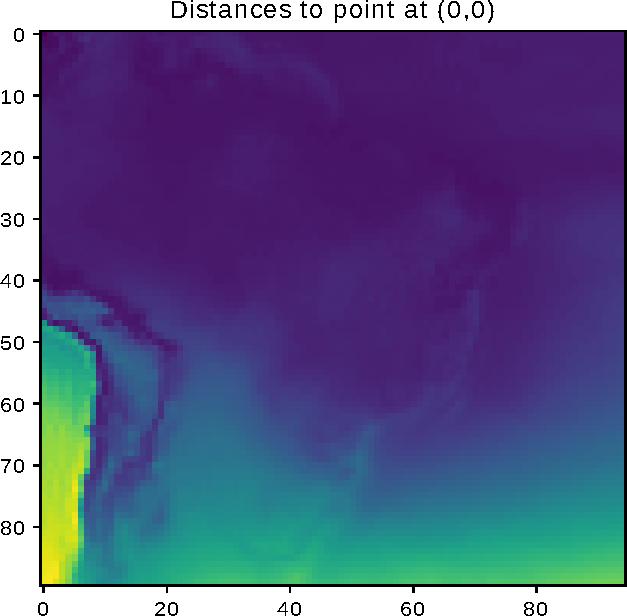
\includegraphics[width=0.45\linewidth]{../Figures/distances_0_0_whole_real_brazil.pdf}
	}
	%no space
	\hfill
	\subfloat{%[DTW distance from the center to the other elements.]{\label{Fig:DTW-DistanceCenter}
		\centering
		
		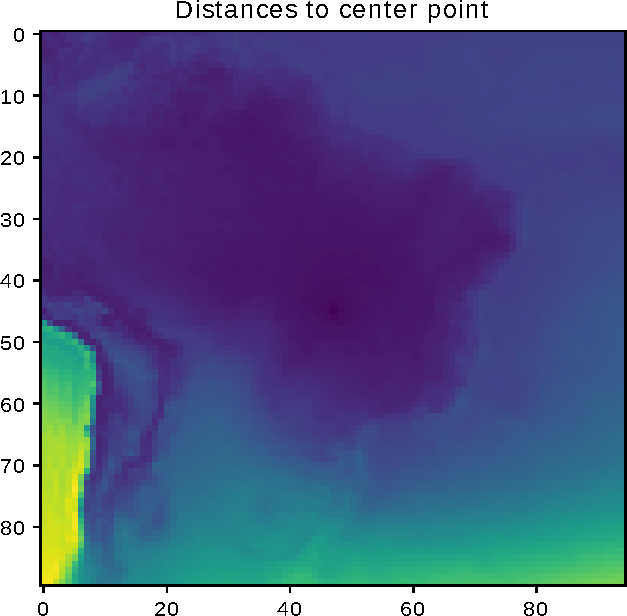
\includegraphics[width=0.45\linewidth]{../Figures/distances_center_whole_real_brazil.pdf}
	}
	\caption{DTW Distance of the time series in the Brazilian region: axes represent spatial indices of the time series, color represents the value of the distance.}
	\label{Fig:DTW-Distance}
\end{figure}

\subsection{Analyzing the Domain Partitioning Techniques}
\label{Sec:AnalyzeDomainPartitioning}

In this Section we describe the experiments performed to validate the strategies adopted for the domain partitioning. We consider two partitioning techniques: $k$--medoids based and regular partitioning; the first groups elements of the domain according to the DTW similarity measure, whereas the second is a partitioning technique based on the geometry of the domain (see Section \ref{Sec:DomainPartitioning} for details). In both approaches, we consider the existence of representative elements for each group, medoid and centroid respectively. 

%TODO when this hypothesis is validated, refer to Section \ref{Sec:AnalyzeDomainPartitioning}
A hypothesis we want to highlight is that it should be preferable to use a partitioning technique that considers grouping domain elements based on the similarity of their temporal evolution, rather than creating groups just according to a regular division of the domain geometry. To verify this, we compare the intra-cluster sum of both partitioning techniques for several values of $k$.

Another important aspect to evaluate in $k$--medoids is the choice of the number of partitions ($k$), for this we use three approaches: elbow method, silhouette index and the inflection point using a smooth spline (see Section \ref{Sec:domain_number_groups} for a description of these methods).

\subsubsection{Evaluating Partitioning Quality}
\label{Sec:EvaluatingPP}

In Sections \ref{Sec:DomainPartitioning} and \ref{Sec:domain_number_groups}, we discussed how we can evaluate the robustness of the $k$--medoids clustering, by comparing its performance with the regular partitioning when varying the number of groups $k$. Here, we describe the experiments used to assess quality of the generated partitions, and analyze the different techniques used to find useful values for $k$.  

For the two partition techniques, we vary the number of groups from $k=2$ up to $k=150$ with a stride of two. In Table \ref{Table:TotalSumRegularkMedoids}, we show the within-cluster sum of squares for both domain partitioning techniques, with $k$ vaying from two to $150$, graphically represented in Figure \ref{Fig:TotalSum-RegularKmedoids}. 
\begin{table}[h]
	\centering
	\tiny
	\begin{tabular}{|c|r|r|c|r|r|c|r|r|}
		\hline
		$k$  & $k$--Medoids & Regular & $k$ & $k$--Medoids & Regular & $k$ & $k$--Medoids & Regular \\ \hline
		2  & 12468.405 & 13190.136 &  52 & 8645.736 & 10032.124 & 102 & 7796.861 &  8855.428 \\
		4  & 11677.377 & 13115.736 &  54 & 8606.070 &  9485.886 & 104 & 7772.689 &  8706.568 \\
		6  & 11218.553 & 12546.427 &  56 & 8566.783 &  9480.166 & 106 & 7752.124 & 12067.876 \\
		8  & 10861.431 & 12517.237 &  58 & 8518.216 & 11466.201 & 108 & 7720.876 &  8404.685 \\
		10 & 10556.589 & 12144.754 &  60 & 8470.036 &  9360.978 & 110 & 7705.371 &  8359.722 \\
		12 & 10320.748 & 11537.237 &  62 & 8432.220 & 11922.456 & 112 & 7676.569 &  8470.927 \\
		14 & 10162.890 & 12038.902 &  64 & 8391.178 &  9238.163 & 114 & 7657.374 &  9012.854 \\
		16 & 10016.352 & 11185.784 &  66 & 8352.620 &  9222.670 & 116 & 7631.154 &  9513.241 \\
		18 &  9874.266 & 11011.460 &  68 & 8315.007 &  9769.658 & 118 & 7612.637 & 11943.777 \\
		20 &  9755.024 & 10864.368 &  70 & 8278.471 &  9148.631 & 120 & 7587.633 &  8276.233 \\
		22 &  9623.499 & 11663.244 &  72 & 8232.783 &  9011.589 & 122 & 7570.840 & 11900.903 \\
		24 &  9539.343 & 10613.759 &  74 & 8203.346 & 11645.734 & 124 & 7547.208 & 10152.428 \\
		26 &  9445.446 & 11741.562 &  76 & 8169.848 &  9864.922 & 126 & 7526.430 &  8218.706 \\
		28 &  9358.812 & 10467.305 &  78 & 8130.028 &  9243.270 & 128 & 7510.721 &  8428.220 \\
		30 &  9279.477 & 10250.783 &  80 & 8101.370 &  8879.863 & 130 & 7485.228 &  8341.508 \\
		32 &  9197.485 & 10305.462 &  82 & 8069.011 & 11478.049 & 132 & 7465.314 &  8149.479 \\
		34 &  9135.674 & 11595.505 &  84 & 8039.939 &  8947.657 & 134 & 7447.742 & 11768.667 \\
		36 &  9083.476 & 10081.895 &  86 & 8014.447 & 11439.713 & 136 & 7431.451 &  8247.420 \\
		38 &  9018.006 & 11685.706 &  88 & 7985.764 &  8719.332 & 138 & 7406.728 &  9136.191 \\
		40 &  8969.207 &  9903.558 &  90 & 7955.133 &  8654.838 & 140 & 7390.761 &  8083.724 \\
		42 &  8902.609 &  9865.422 &  92 & 7922.941 & 10004.969 & 142 & 7366.944 & 11675.846 \\
		44 &  8856.496 &  9990.224 &  94 & 7906.157 & 12251.765 & 144 & 7352.245 &  8126.600 \\
		46 &  8795.638 & 11808.071 &  96 & 7884.088 &  8642.817 & 146 & 7333.966 & 11621.432 \\
		48 &  8740.765 &  9653.982 &  98 & 7855.217 &  8773.346 & 148 & 7311.080 &  9715.298 \\
		50 &  8698.159 &  9605.287 & 100 & 7822.593 &  8525.302 & 150 & 7293.661 &  7932.553 \\ \hline
		
	\end{tabular}
	\caption{Total Within cluster Sum of Squares of $k$--Medoids and Regular Partitioning Techniques for $k = \{2, \ldots, 150\}$.}
	\label{Table:TotalSumRegularkMedoids}
\end{table}

\begin{figure}[h]
	%	\begin{minipage}[b]{0.8\textwidth}
	\centering
	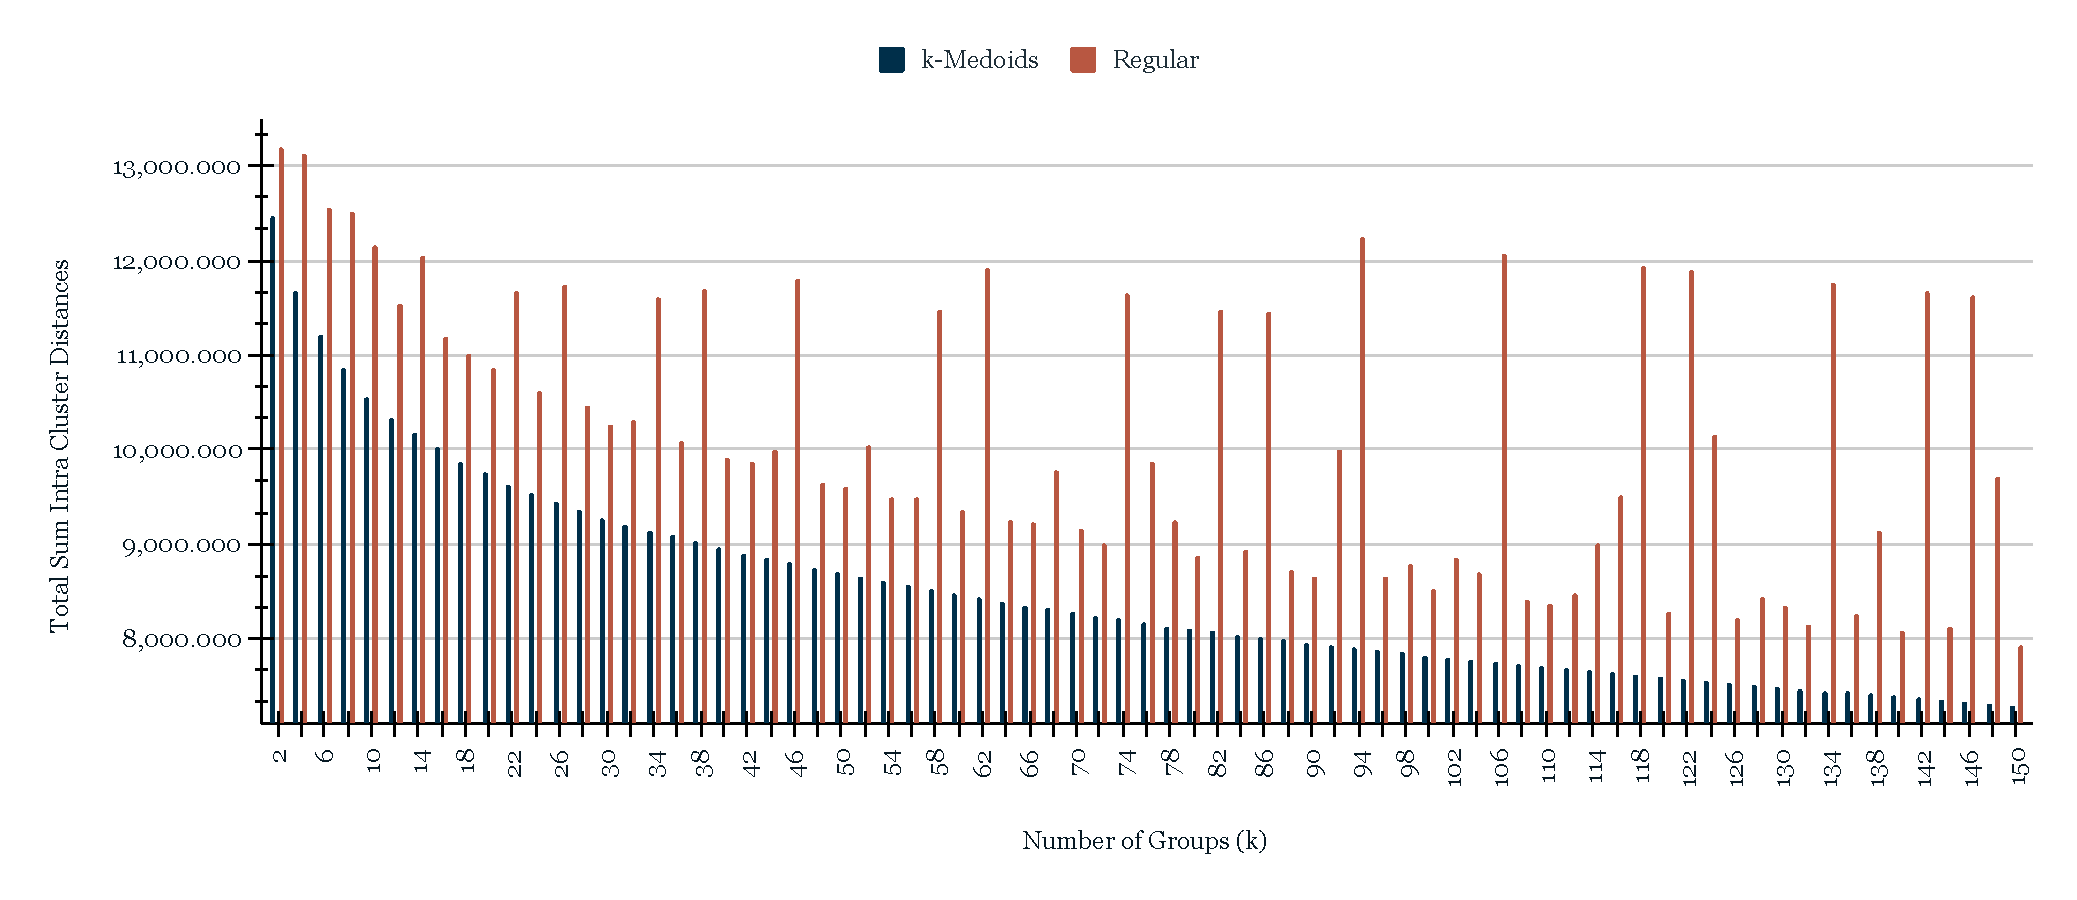
\includegraphics[scale=0.46]{../Figures/Scaled-TotalSum-RegularKmedoids}
	\caption{Total Within cluster Sum of Squares of $k$--Medoids and Regular Partitioning Techniques.}
	\label{Fig:TotalSum-RegularKmedoids}
	%	\end{minipage}
\end{figure}

In the previous figure, it is possible to observe the decreasing behavior of the WSS curve (see Section \ref{Sec:kMedoidsClustering}) for higher values of $k$. In clustering, the goal is not only create cluster from the dataset, but create more accurate clusters that can be use to generate insights about the characteristics of the dataset.

\subsubsection{Selecting $k$}
\label{Sec:Selectk}

% Methods to select k
The $k$--medoids algorithm requires the user to specify $k$, the number of clusters to be generated. When using a clustering technique for high volumes of data and low variability of the data values throughout neighbor points, it is difficult to determine the optimal number of groups. This is particularly important for our problem, where there is low variation in the spatial data distribution of the different time series. In Section \ref{Sec:domain_number_groups}, some methods for determining suitable values for $k$ were discussed. Here, we show the results of applying these methods to our case study as part of the Step 1 of our methodology (Section \ref{Sec:DomainPartitioning}) in order to determine the partioning schemes that will be used in the later steps.

One common method of choosing the appropriate cluster solution is to compare the Within-Sum-of-Squares (WSS) for a number of cluster solutions. Thus, WSS can be seen as a global measure of error. In general, as the number of clusters increases, the WSS should decrease because clusters are consequently smaller. A plot of the WSS against a series of sequential cluster levels can provide a useful graphical way to choose an appropriate cluster level. An appropriate cluster solution could be defined as the solution at which the reduction in WSS slows dramatically. This produces an ``elbow'' in the plot of WSS against cluster solutions. 

For our dataset we find an ``elbow'' at the four cluster solution suggesting that solutions greater than four do not have a substantial impact on the total sum of square errors, Figure \ref{Fig:SSE-kMedoids} shows this result. The low number of groups indicated by the elbow method is consistent with the observation (see Figure \ref{Fig:DTW-Distance} and corresponding discussion) that there is a low variability of the temporal data values throughout neighbor points, but which accumulate to produce larger variability throughout the region.

% TODO bigger fonts
\begin{figure}[h]
	%	\begin{minipage}[b]{0.8\textwidth}
	\centering
	\includegraphics[scale=0.5]{../Figures/Elbow-Kmedoids}
	%\caption{Elbow Method to find the optimal $k$ for the $k$--Medoids Approach.}
	\caption{Application of the Elbow Method, optimal $k=4$ highlighted in red.}
	\label{Fig:SSE-kMedoids}
	%	\end{minipage}
\end{figure}

When performing a Silhouette Analysis, a way to measure how close each point in a cluster is to the points in its neighboring clusters. We want to maximize the value of the silhouette score, which would indicate that each sample belongs strongly to its own cluster as opposed to a neighboring cluster.

For the temperature dataset, we performed the silhouette analysis to calculate the score for the range of values of $k$ described in the previous Section. The results are in Figure \ref{Fig:Silhouette-kMedoids}, and the maximum score was $0.145$ which corresponds to $k = 8$. 

In general, we obtained low values for the silhouette score throughout the considered range of $k$, indicating that, for high values of $k$, the samples are weakly belonging to its own cluster and could also be matched with neighboring clusters. Again, this is an indication that there is low variability throughout neighboring points.

\begin{figure}[h]
	%	\begin{minipage}[b]{0.8\textwidth}
	\centering
	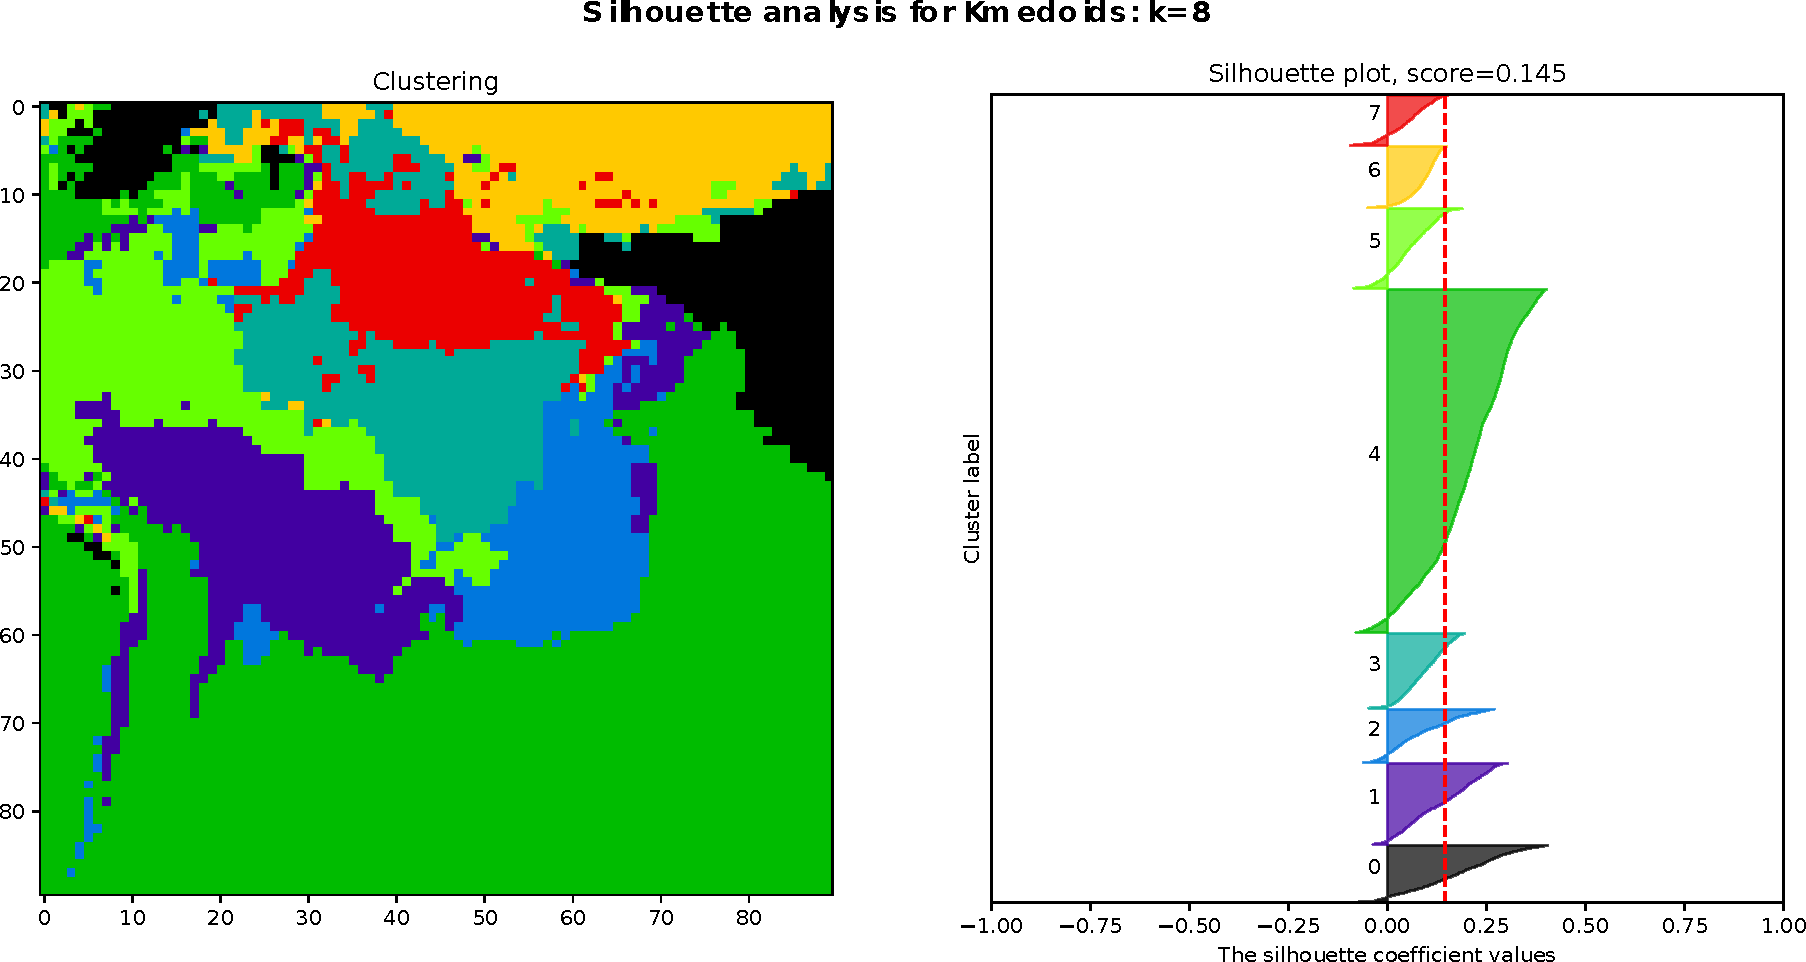
\includegraphics[scale=0.50]{../Figures/silhouette-kmedoids_k8_seed0_lite}
	%\caption{Silhouette Index for $k=8$.}
	\caption{Application of the Silhouette Analysis, showing $k=8$ with highest silhouette index.}
	\label{Fig:Silhouette-kMedoids}
	%	\end{minipage}
\end{figure}

An additional method to find the optimal value for $k$, based on the inflection point, consists in fitting the values of total sum of intra cluster distances using a cubic smooth spline. We are interested in finding the point where the curvature of the fitted model is the maximum \cite{Akima1970}. The results for our dataset are shown in Figure \ref{Fig:SmoothSpline-kMedoids}, and the computed value is $k = 66$.

We argue that this method is more appropriate for our dataset, in contrast to the previous two methods, as it highlights the decreasing trend in the intra-cluster cost as $k$ increased. This was possible because the small variations, that were preventing the other methods to find a higher value for $k$, were smoothed by the splines.

\begin{figure}[h]
	%	\begin{minipage}[b]{0.8\textwidth}
	\centering
	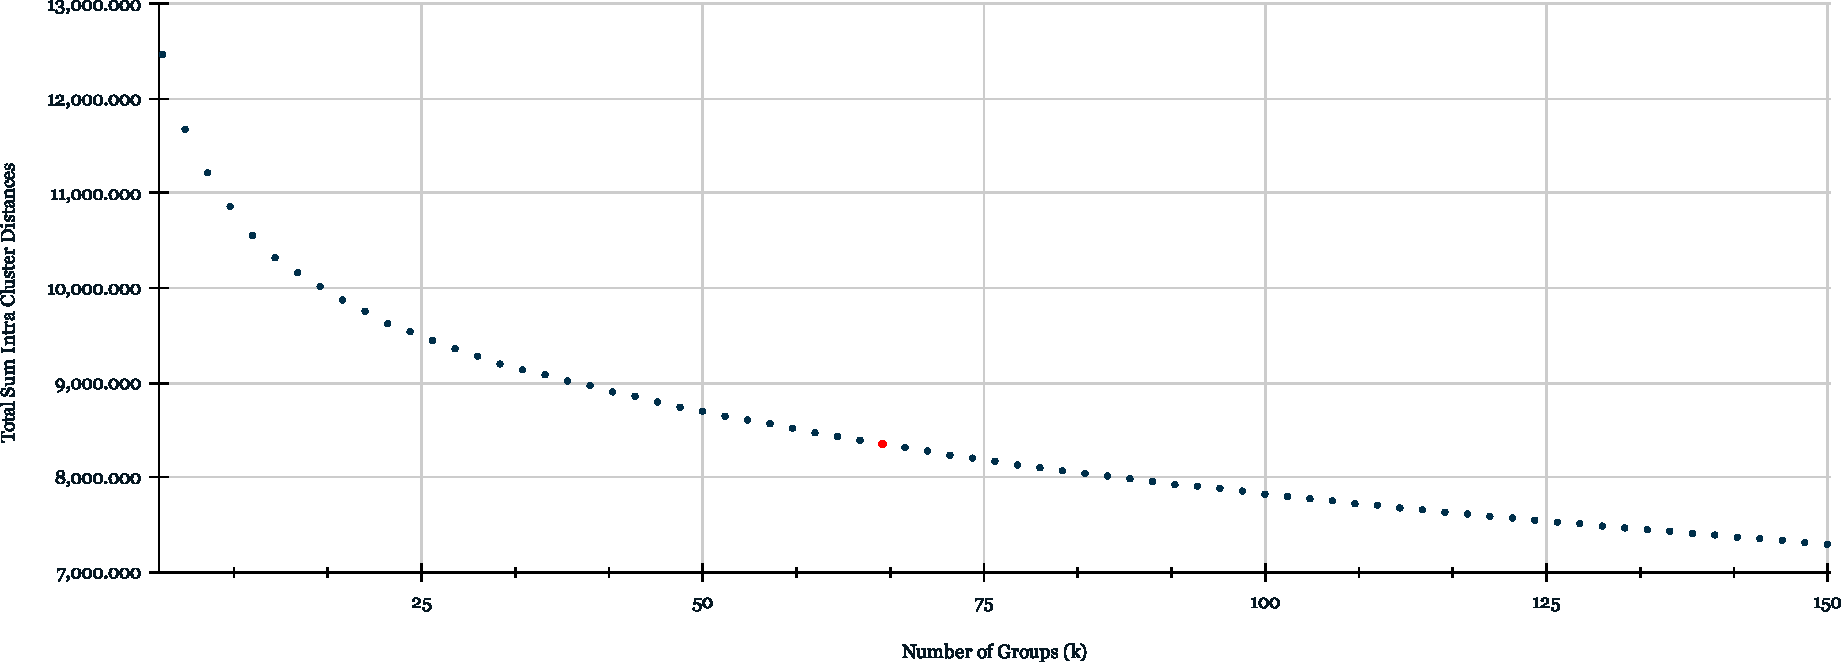
\includegraphics[scale=0.5]{../Figures/SmoothSpline-kMedoids}
	%\caption{Smooth Spline Fitting Method to find the optimal $k$ for the $k$--Medoids Approach.}
	\caption{Application of the Spline Fitting Method, optimal $k=66$ highlighted in red.}
	\label{Fig:SmoothSpline-kMedoids}
	%	\end{minipage}
\end{figure}

We observe that several methods to find an optimal value for $k$ give us different values. Figure \ref{Fig:OptimalkKMedoids} shows the resulting groups when applying two of these partitioning techniques; the marks indicate the representative points of each group. 
% TODO Argumentar que puede estar pasando
Table \ref{Table:ValidationIndex} summarizes the findings of applying the available methods to find optimal values for $k$.
\begin{table}[h]
	\centering
	\small
	\begin{tabular}{|l|c|}
		\hline
		Method & Optimal $k$ \\ \hline
		Elbow  & 4	\\
		Silhouette & 8	\\
		Smooth Spline for SSE & 66\\ \hline
	\end{tabular}
\caption{Methods to find the optimal value for $k$.}
\label{Table:ValidationIndex}
\end{table}
		
\begin{figure}[htb]
	\centering
	\subfloat{%[DTW distance from the point $(0,0)$ to the other elements.]{\label{Fig:DTW-Distance0}
		\centering
		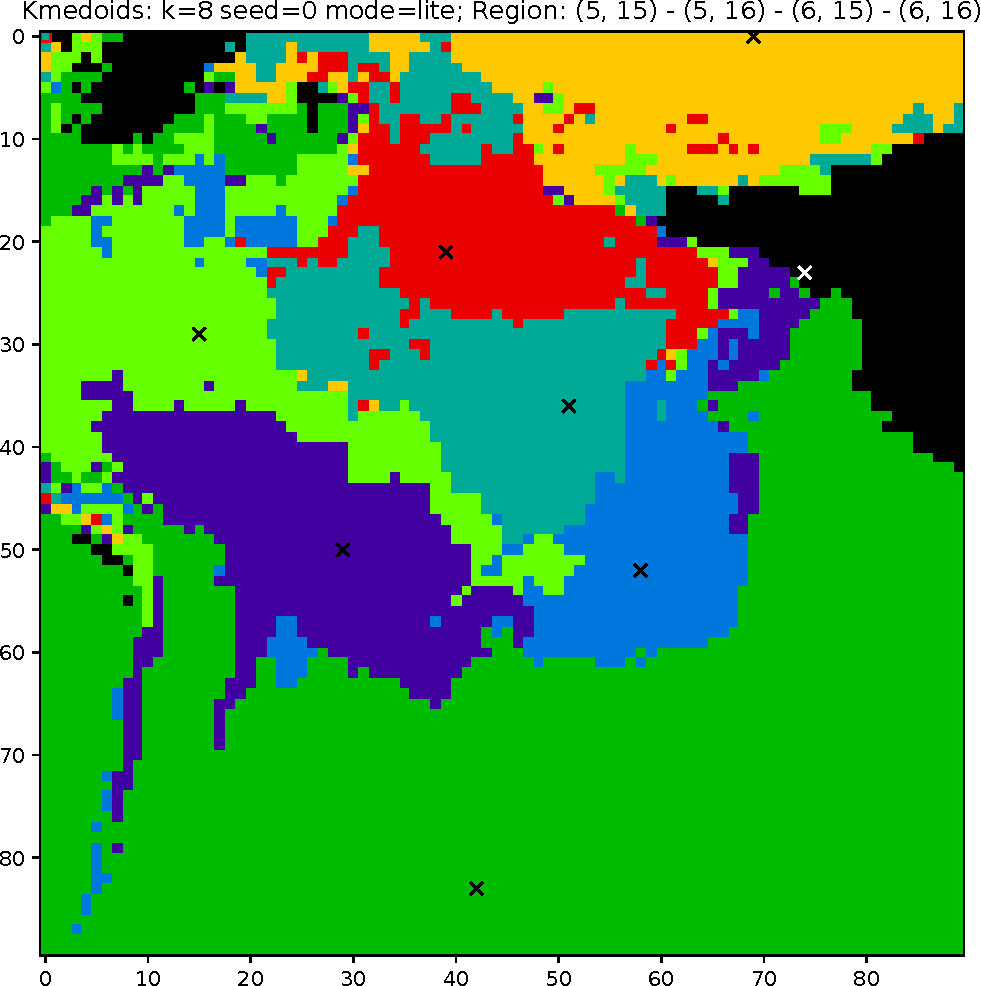
\includegraphics[width=0.45\linewidth]{../Figures/query-kmedoids_k8_seed0_lite__region-0-1-0-1}
	}
	%no space
	\hfill
	\subfloat{%[DTW distance from the center to the other elements.]{\label{Fig:DTW-DistanceCenter}
		\centering
		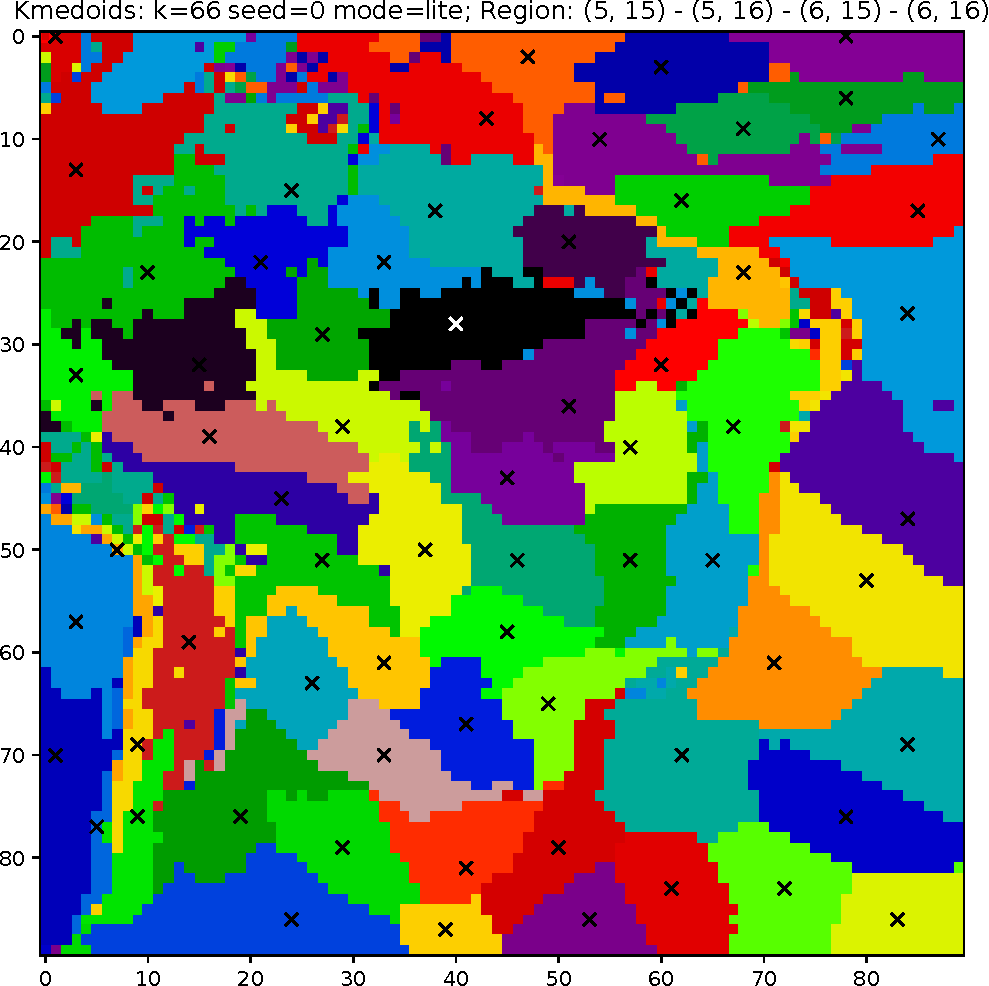
\includegraphics[width=0.45\linewidth]{../Figures/query-kmedoids_k66_seed0_lite__region-0-1-0-1}
	}
	
	\caption{Groups obtained with $k$--Medoids using $k=8$ (left) and $k=66$ (right). Corresponding medoids are marked with a `$\times$'.}
	\label{Fig:OptimalkKMedoids}
\end{figure}	

\subsubsection{Discussion on Domain Partitioning}
\label{Sec:DomainPartitioningDiscussion}

% Justification and Summarization
Spatial-temporal data are heterogeneous and autocorrelated, consequently the data are consistent and smoothly variable \cite{}. The division of the domain into $k$ parts by a method that considers the similarity in the temporal evolution of its elements is indeed superior to a method that does not consider any similarity. Furthermore, there is more than one $k$ that, based on temporal similarity, expresses better different regions of the domain.

The evaluation of this part of the methodology allowed us to establish the $k$--medoids algorithm as a significantly superior partitioning solution, compared to the naive approach of a regular partitioning used as baseline. This was demonstrated even when increasing the number of groups: while both partitioning algorithms exhibit a decreasing trend in the sum of intra-cluster distances (partitioning cost), the cost of the $k$--medoids algorithm was consistently smaller than the baseline. Also, the trend was monotonous for $k$--medoids, while it showed variability for the regular partitioning (the latter variability can be explained by the arithmetic of dividing the region in equal rectangles). 

The monotonous trend of $k$--medoids allowed for the calculation of the inflection point, which effectively calculated a high value for $k$ to represent a suitable partitioning scheme ($k = 66$). This value gives us a reasonable number of representatives that we can use in the next phases of the methodology. Also, since we applied two other validation methods for selecting $k$ that produced two other domain partitioning schemes, we can also consider these groups and their representatives when evaluating a model composition. 

% DBSCAN - Not included in the final version to avoid confusion or off-topic discussions.
%In addition to $k$--Medoids, we also explored DBSCAN, another clustering method that can also use DTW as the similarity measure. DBSCAN is a procedure to find `optimal' number of groups based on the spatial density of the data, and uses two parameters: the maximum ray to agglomerate points and the minimum number of elements per group. Its disadvantage is that being an algorithm that only finds convex groups, if the elements are not similar they are considered outliers. When DBSCAN was applied to our dataset, it would either find only two groups containing most of the data points, or few groups that failed to contain most of the points, because DBSCAN would mark other points as outliers. After this exploration of DBSCAN, further analysis with it was discontinued.

In the following section, we describe the process to generate predictive models on the representative elements and the experiments to evaluate its predictive quality.

\subsection{Forecast Error Analysis of Predictive Models on Representatives}
\label{Sec:AnalyzePredictorRepresentatives}

% Objective: Evaluate that it is sufficient to use a models over a group representative for every group element.
In this section we perform extensive experiments to evaluate the predictive power of models trained on the representative elements of each group. 
% TODO: GM Revisar escrita y tal vez cambiar el orden del texto.... 
One of the main reasons we adopt this approach is because we intend to accelerate the computational intensive process involved in perform the forecast of multiple time series, in some cases too many to analyze manually.

% Predictor ARIMA
Following the Step two of our proposed methodology (Section \ref{Sec:ModelRepresentatives}), we generate an ARIMA model for each representative obtained from the domain partitioning. We denote the subset of representative elements for different values of $k$ by $\mathbf{R} \subset \mathcal{D}$, and the generated models $g$ as per equation \ref{eq:ModelDefinition}, $g \in \mathcal{G}_{(\mathbf{R})}$. 

In this context, the model parameters $\mathbf{p}$ comprise both the ARIMA $(p, d, q)$ parameters, and the default hyper-parameters used in an implementation of \texttt{auto.ARIMA}\footnote{\texttt{auto.ARIMA}: Implementation on \url{https://robjhyndman.com/publications/automatic-forecasting/}} that finds a suitable tuple $(p, d, q)$, as described in Section \ref{Sec:TheoryARIMA}. A predictive model is then completely characterized by the $(p, d, q)$ tuple and the series used as training data. 
% TODO Add the importance of the residuals
% Residuals are useful in checking whether a model has adequately captured the information in the data. A good forecasting method will yield residuals with the following properties: The residuals are uncorrelated.

The prediction intervals, which are a way to display the uncertainty in forecasts, for ARIMA models are based on assumptions that the residuals are uncorrelated and normally distributed. 

% Evaluate the prediction interval of the representatives (in-sample)
% Trade-off between the representative model accuracy and the computational intensive process to perform the creation of model for every element in the domain.

\subsubsection{Obtaining In-sample and Forecast Errors}
\label{sec:InSampleForecastErrors}

% Analyze the in-sample error for the representatives first, later use an argument similar to the NFLT for time-series. Using the in-sample error of the model on the representatives for series within each group
Figure \ref{Fig:TimeSplit} shows the division of time units on the time series in order to train and test an ARIMA model. Recalling the preparation of the dataset described in Section \ref{sec:DatasetPreparation}, we work with 365 values for each representative point, denoted by the series $s[0:364]$.

\begin{figure}[h]
	\centering
	\includegraphics[scale=0.38]{../Figures/ModelRegion_ModelTS}
	\caption{Time units split for training and test datasets.}
	\label{Fig:TimeSplit}
\end{figure}

Let's consider a particular representative $\mathcal{S}^{*} \in \mathbf{R}$ and its associated temperature series $s_r$. To evaluate an ARIMA model $g_{s_r}$ and its predictive power, the series is then split into three parts. The first part is used for training the model ($s^t_r[0:349]$ as an example in Figure \ref{Fig:Time-SeriesSplit}), here we determine the tuple $(p_{s_r}, d_{s_r}, q_{s_r})$ that corresponds to the model $g_{s_r}$. Then, we take the next $t_p$ data points ($t_p = 8$ in our example) to create the validation series $s^v_t[349:357]$. The purpose of this subset is to obtain the in-sample error ${E^*}$ of the model: this is achieved by using the model $g_{s_r}$ to make a prediction of $t_p$ steps, and then calculating an associated error using one of the error expressions presented in Section \ref{Sec:ModelRepresentatives}.

\begin{figure}[h]
	\centering
	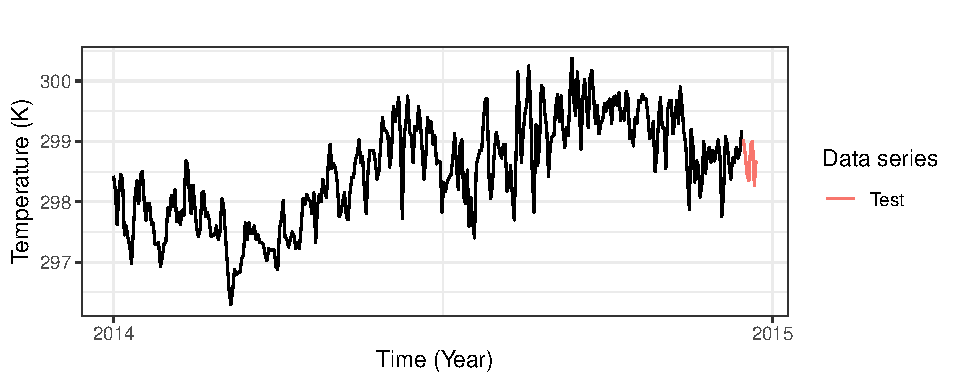
\includegraphics[scale=1]{../Figures/medoid_test_training}
	\caption{Dataset Split for a Time Series Representative ($s^t_r$ in black, $s^v_t$ in pink).}
	\label{Fig:Time-SeriesSplit}
\end{figure}

To enable forecasting, the model is retrained using the same $(p, d, q)$ model parameters found with $s^t_r$, but now using a longer series $s[0:357]$ (previous training series now extended with the validation series). In order to evaluate the model's predictive power, we use it to forecast $t_f$ steps into the future ($t_f = 8$ in our example) that the model has not seen. But, since the subset $s[357:364]$ is actually available from the dataset, we are evaluate to calculate the forecast error, allowing us to perform forecast error analysis on different representatives from different domain partitioning schemes. 
%The error analysis described can also be applied to the $k$NN predictive model (baseline).

In order to show this approach in action, we present Figure \ref{Fig:ModelFinalToForecast}, where we show the ARIMA model with parameters $(3,1,1)$ for a medoid in a domain partitioning ($k=8$). Represented with a blue line, we have the forecast values for $t_{f} = 8$, while the prediction intervals with $95\%$ and $80\%$ confidence levels are shown in blue and light blue shades, respectively. The values fitted by the model are also shown in pink, on top of the original time series for the retrained model in black.

\begin{figure}[h]
	\centering
	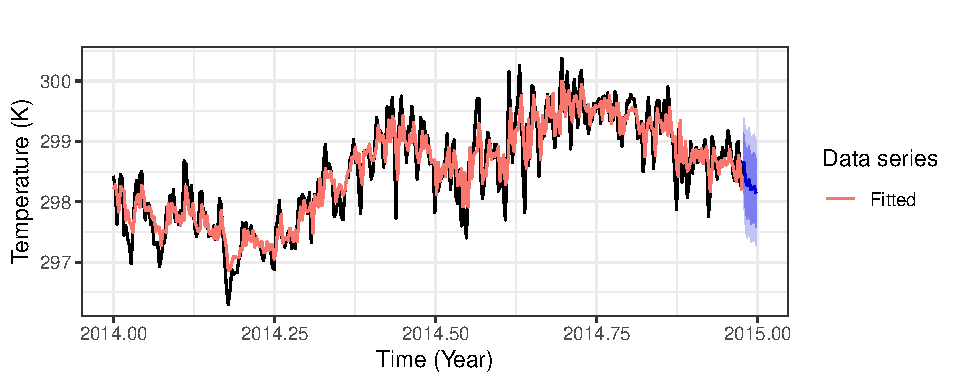
\includegraphics[scale=1]{../Figures/medoid_forecast_fitted}
	\caption{Forecast, fitted.}
	% Change caption.
	\label{Fig:ModelFinalToForecast}
\end{figure}

% Forecast estimates are provided with confidence bounds: 80% confidence limits shaded in darker blue, and 95% in lighter blue. For stationary models (i.e., with d=0), forecast intervals converge, for d>1, the forecast intervals will continue to grow into the future.
% Add justification for ARIMA models

\subsubsection{Analyzing Forecast Errors}
\label{Sec:AnalyzeForecastErrors}

% GM Review paragraph
One of the assumptions in the methodology proposed is that we opt for an automated time series forecasting with a reduced number of models, the purpose is perform a forecast for multiple time series inside a region of interest. Therefore this models used for forecasting must be able to fit to times series in different regions of the domain. It is known that is almost impossible to find the best model for each and every single time series \cite{HastieTF2009}, but using our approach, these reduced number of models are reasonable good on average over all the time series, also it is possible that for some of those time series could exists better models that those considered for the representatives.

% Add comparison important, for elements (other than representatives) compare the actual values with the forecast and prediction intervals of the representative. 
% GM review paragraph
Comparison of forecast prediction intervals for the representative element model when is used in another element in their group. In the case of a $k=8$, we have groups with the number of elements varying from 500 to 3479, representing the $6.2\%$ and $43\%$ of the domain respectively. This means that exists eight models that could perform reasonable good predictions for any element in the domain.

% Add the forecast 
\begin{figure}[h]
	\centering
	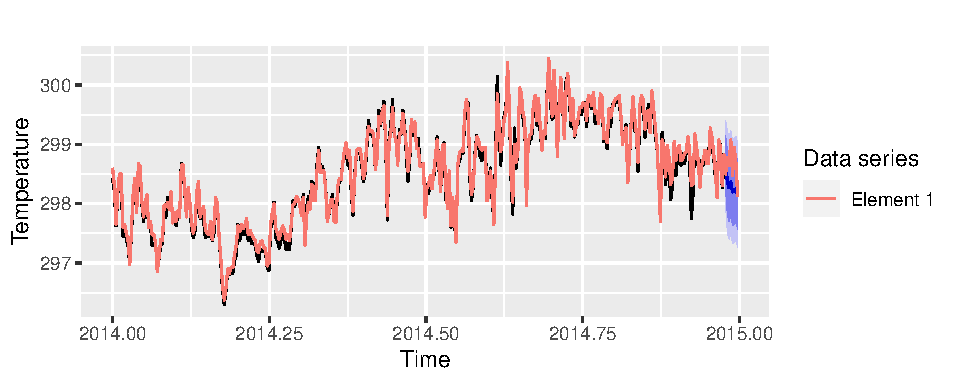
\includegraphics[scale=1]{../Figures/forecast_element1}
	\caption{Forecast, fitted.}
	% Change caption.
	\label{Fig:ForecastElement1}
\end{figure}


% GM review paragraph....
By considering a greater value for the number $k=66$, we are creating more groups and therefore more representatives that generalize better the elements in its group. The partitioning domain result are groups varying from 14 to 278 elements, representing the $0.2\%$ and $3.4\%$ of the domain respectively.

% Forecast Error vs. DTW distance intra-cluster
% Main objective: Within a group, evaluate the variation of the forecast error obtained when the model is applied over all the elements in the group. In practice we are computing the value forecast on the representative for $t_f = 8$, then we compute the sMAPE using the observational values on the representative.

Given that the prediction intervals for the forecast of the model built using the representative element are varying values between the forecast error of the model composition listed, we need to analyze the intra cluster variability. When applying $k$--medoids to the domain, the number of elements on each cluster are different and it is not feasible to find a significant correlation between the model composition forecast error and the DTW distance from the medoid.

% TODO Re-make figures with the same scale for k =8 and k=66, using the same scale for the forecast errors. Compute the amount of points with `low' or `close' forecast error compared with the medoid forecast error (use percentage or $\pm$ values).

% Figures 
% DTW Maximum 2.5 

% Maximum Forecast Error 1.0 
\begin{figure}[!tbp]
  \centering
  \begin{minipage}[b]{0.45\textwidth}
    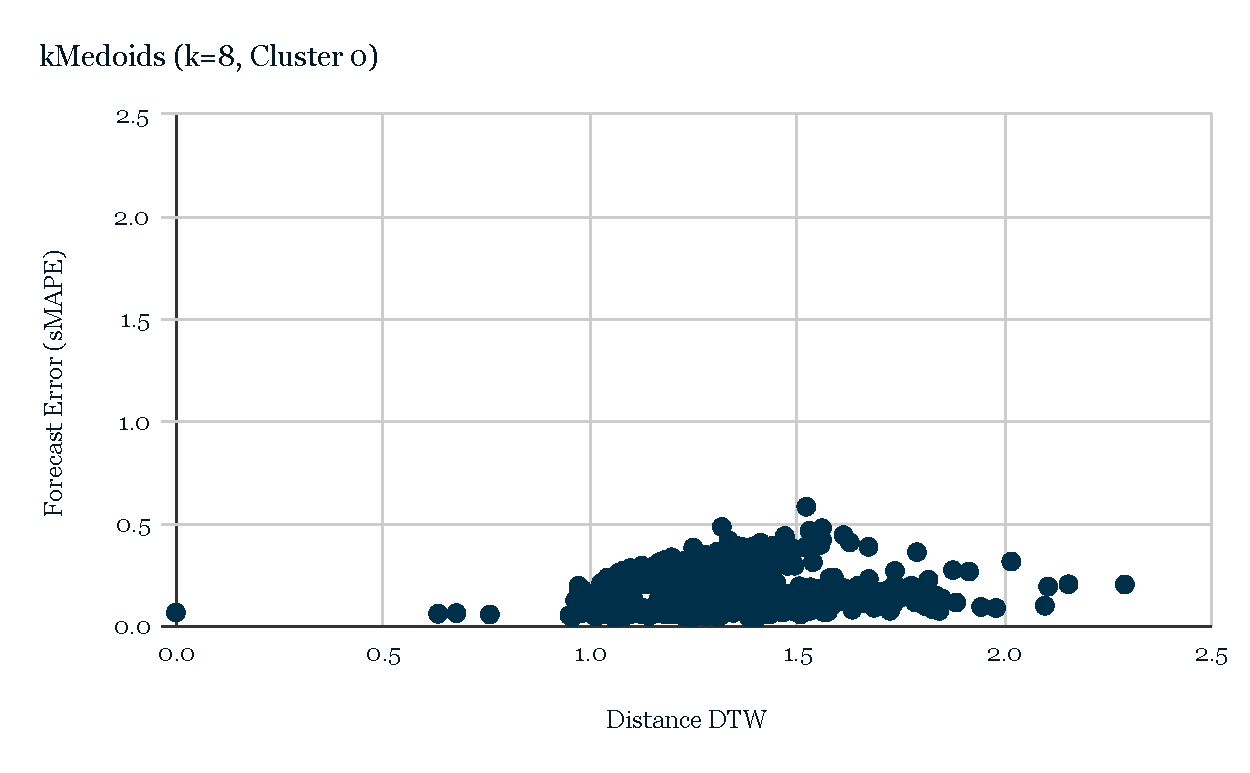
\includegraphics[width=\textwidth]{../Figures/distDTW_ForecastError_k8_c0}
    \caption{Flower one.}
    \label{Fig:Test1}
  \end{minipage}
  \hfill
  \begin{minipage}[b]{0.45\textwidth}
    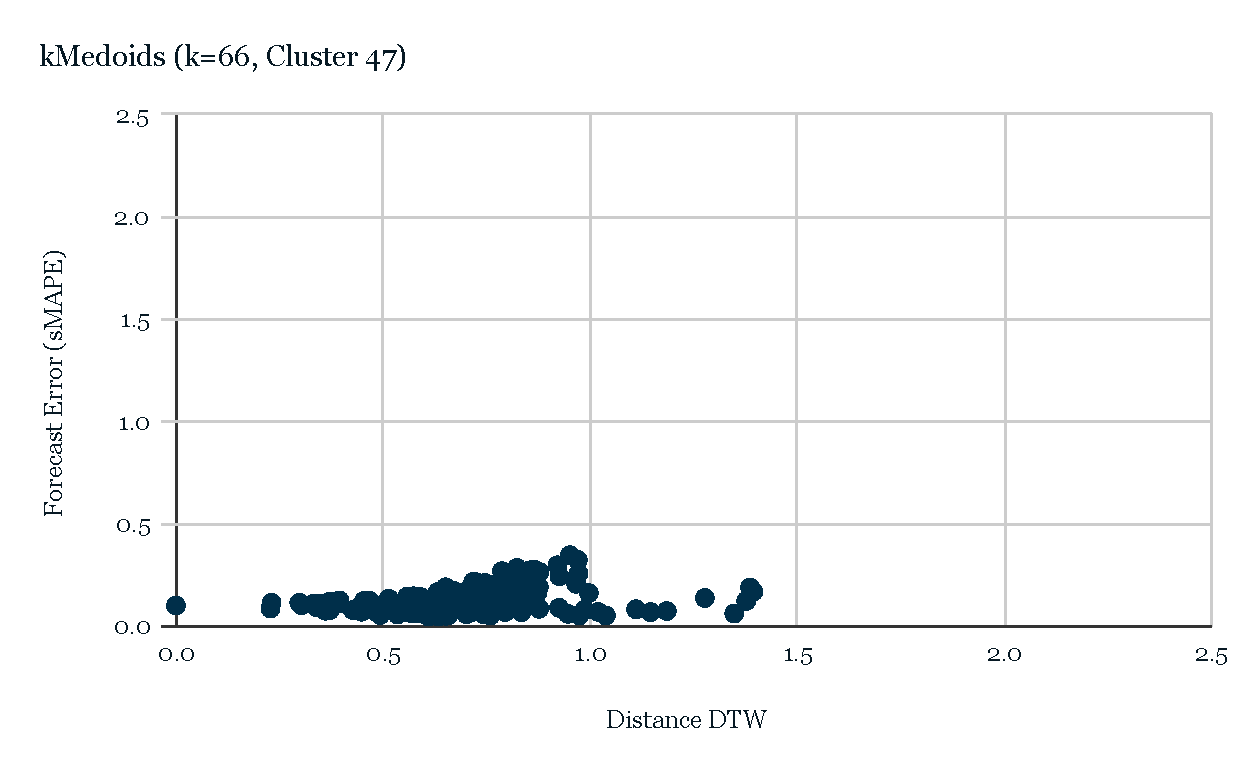
\includegraphics[width=\textwidth]{../Figures/distDTW_ForecastError_k66_c47}
    \caption{Flower two.}
    \label{Fig:Test2}
  \end{minipage}
\end{figure}

% Maximum Forecast Error 1.5

\begin{figure}[!tbp]
  \centering
  \begin{minipage}[b]{0.45\textwidth}
    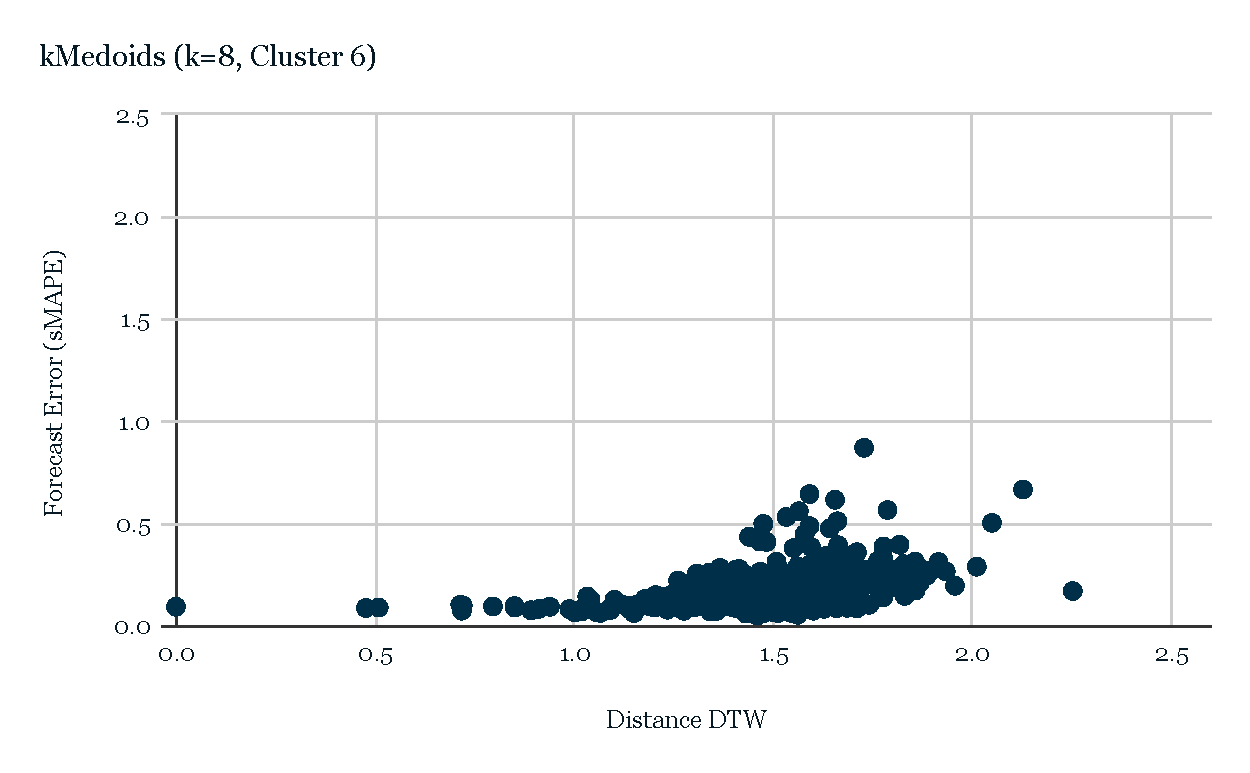
\includegraphics[width=\textwidth]{../Figures/distDTW_ForecastError_k8_c6}
    \caption{Flower one.}
    \label{Fig:Test1}
  \end{minipage}
  \hfill
  \begin{minipage}[b]{0.45\textwidth}
    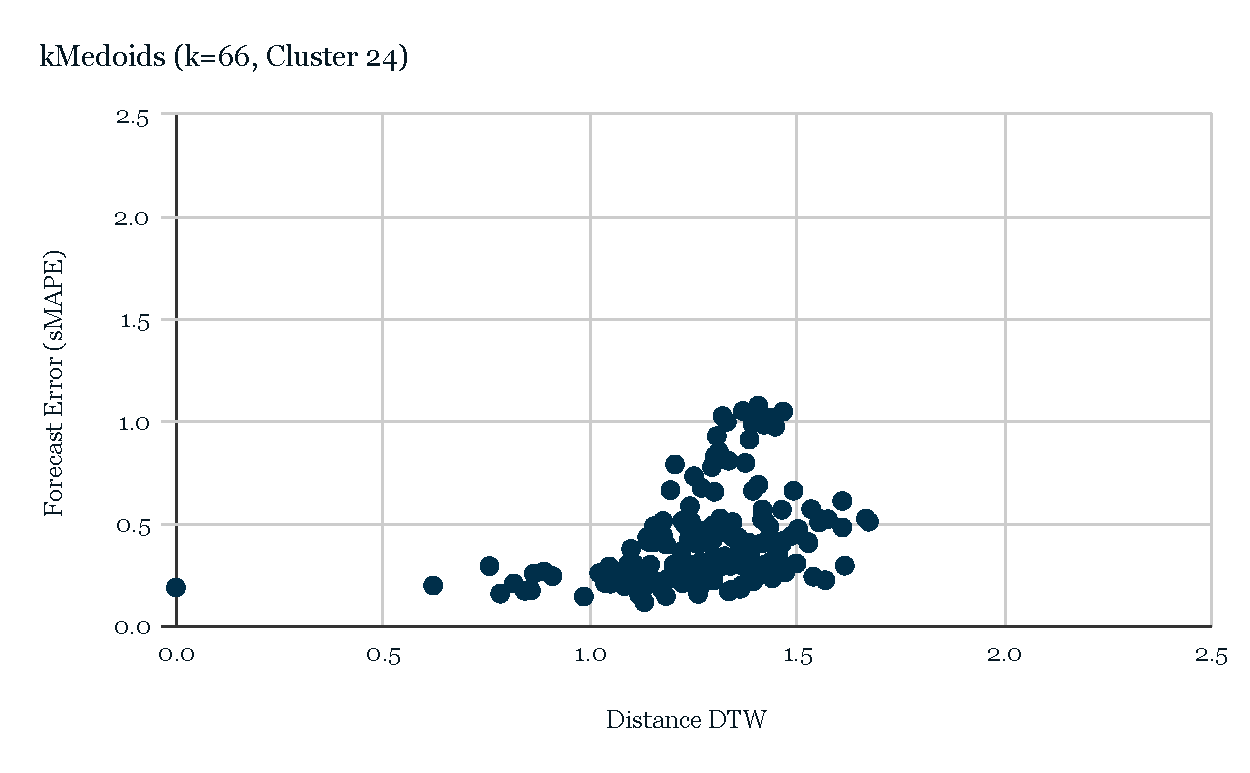
\includegraphics[width=\textwidth]{../Figures/distDTW_ForecastError_k66_c24}
    \caption{Flower two.}
    \label{Fig:Test2}
  \end{minipage}
\end{figure}

% Maximum Forecast Error 2.0

% Maximum Forecast Error 2.5

% Para evaluar cuantitativamente el poder predictivo de la forecast con t_f=8 
To quantify individually the predictive power of the representative predictor forecast error, we compute the sMAPE of each element 




% Conclusion: It is not feasible to find a direct correlation between DTW distance and forecast error (and also in-sample error), this is due to the nature of the ARIMA models (elaborate more). To establish a more generic function for the forecast error, or the predictive power, we have to consider 
% TODO Add reference for the statistical equivalent of the learning function.


 As a part of the off--line process we store the resultant predictive models, this will allow us to speed--up the task of compute a forecast for a time series.
 
\subsubsection{Predictive Quality of Model Composition}
\label{Sec:ModelComposition}

% We are using a model on a representative element, one that generalizes the temporal evolution of a group contained in the study domain. We want to evaluate the prediction error 'in-sample' of the model applied on the other elements, we seek to find a balance between the minimum and maximum error of the 
We are interested in evaluate the forecast error for a model composition, as discussed in Section \ref{Sec:KnowledgExtraction} of the methodology. A model composition is formed by one or more predictors which will be used to perform a prediction on a domain region. Recalling from Section \ref{Sec:ModelRepresentatives}, the model compositions of interest are:

\begin{itemize}%[noitemsep,nolistsep]
	\item Model Composition with Minimal Error (coded `Min.'): for each group in a partitioning scheme, we find the predictive model that minimizes the accumulated forecast error in the group. 
	\item Model Composition with Minimal Local Error (coded `Min. Local'): naive approach where each time series gets its own predictive model.
	\item Model Composition at the Medoids (coded 'Medoid'): for each group, generate a predictive model and apply it to each point in the group.
	\item Model Composition with Maximum Error (coded `Max.'): for each group, we find the predictive model that maximizes the accumulated forecast error in the group.
\end{itemize}

For each of the model compositions above, we perform the forecast error analysis discussed in Section \ref{Sec:AnalyzeForecastErrors} with one of the associated error metrics described in Section \ref{Sec:TimeSeriesForecast}. Here, we focus on using the sMAPE error metric.

% Forecast Error in a group using the representative predictor.
In the previous step we consider maintain several domain partitioning schemes. Considering the values for $k = \{8, 66, 132\}$, we compute the forecast error of the model compositions listed above, applied over its group generated in the partitioning technique. %In the following tables we 
%TODO Add time to compare
\begin{table}[h]
	\centering
	\tiny
	\begin{tabular}{|c|r|r|r|r|r|r|r|r|r|}
		\hline
		cid & size & $(p, d, q)$ & T. F. (seg) & T. T. (seg) & Each & Min. & Min. Local & Medoid & Max. \\
		\hline
		0 &  990 & (2, 1, 2) & 1.642 & 3601.959 & 0.333 & 0.305 & 0.379 & 0.331 & 0.826 \\
		1 &  990 & (0, 1, 2) & 1.665 & 3221.489 & 0.192 & 0.180 & 0.198 & 0.268 & 0.517 \\
		2 &  990 & (1, 1, 2) & 1.621 & 4063.693 & 0.384 & 0.460 & 0.888 & 0.587 & 1.608 \\
		3 &  990 & (2, 1, 1) & 1.610 & 3424.456 & 0.341 & 0.387 & 0.634 & 0.394 & 1.028 \\
		4 &  990 & (2, 1, 2) & 1.651 & 4305.636 & 0.782 & 0.571 & 1.182 & 0.769 & 3.058 \\
		5 &  990 & (1, 1, 2) & 1.713 & 3818.287 & 0.470 & 0.489 & 0.580 & 0.609 & 2.062 \\
		6 & 1080 & (0, 1, 0) & 1.744 & 4674.208 & 1.190 & 0.564 & 0.862 & 2.454 & 2.935 \\
		7 & 1080 & (2, 1, 1) & 1.795 & 4847.003 & 0.546 & 0.463 & 0.563 & 0.583 & 1.188 \\ \hline
	\end{tabular}
	\caption{Model Composition Forecast Error for Regular Partitioning with $k=10$.}
	\label{Table:ForecastErrorRegulark10}
\end{table}

In Table \ref{Table:ForecastErrorRegulark10}, the parameters $(p, d, q)$ and  AIC correspond to the ARIMA predictor for the time series representative. Here, we use the code for each model composition described above; T.F is the elapsed forecast time for eight time units and T.T is the total time used for training and forecast. 

\begin{table}[h]
	\centering
	\tiny
	\begin{tabular}{|c|r|r|r|r|r|r|r|r|r|}
		\hline
		cid & size & $(p, d, q)$ & T. F. (seg) & T. T. (seg) & Each & Min. & Min. Local & Medoid & Max. \\
		\hline
		0 &  574 & (0, 1, 2) & 1.069	&  2041.469	& 0.170	& 0.161	& 0.289	& 0.185	& 0.438	 \\
		1 &  817 & (2, 1, 2) & 1.299	&  3447.608	& 0.689	& 0.460	& 0.531	& 0.926	& 1.566	 \\
		2 &  542 & (1, 1, 2) & 0.880	&  2011.441	& 0.581	& 0.514	& 0.577	& 0.678	& 1.420	 \\
		3 &  755 & (1, 1, 1) & 1.238	&  2685.912	& 0.413	& 0.289	& 0.364	& 0.492	& 0.878	 \\
		4 & 3479 & (1, 1, 2) & 5.727	& 14542.318	& 0.785	& 0.475	& 0.548	& 0.838	& 1.983	 \\
		5 &  803 & (1, 1, 1) & 1.375	&  3231.718	& 0.407	& 0.294	& 0.378	& 0.437	& 1.194	 \\
		6 &  625 & (3, 1, 1) & 0.957	&  1930.740	& 0.157	& 0.168	& 0.175	& 0.203	& 0.478	 \\
		7 &  505 & (3, 1, 1) & 0.853	&  1811.335	& 0.388	& 0.375	& 0.422	& 0.551	& 1.015	 \\ \hline	
	\end{tabular}
	\caption{Model Composition In-Sample Error for Partitioning Technique  $k$--Medoids with $k=8$ and \texttt{seed = 0}.}
	\label{Table:ForecastErrorkMedoidsk8}
\end{table}

% Analyze the prediction error for solvers in a region 10x10 when varying k
For the $k$--medoids partitioning we compute the same values for $k=8$, shown in Table \ref{Table:ForecastErrorkMedoidsk8}. Experimentally, we can see that when considering the prediction of the medoid as the prediction for the points of its group, there is a balance in the final prediction value in the analyzed region. This ensures that we can use the medoids and their respective predictive models to predict the time evolution of the entire domain.

For each $k$ considered, it is possible to observe that the predictions made by the models in the medoids are lower, this is due to the fact that the points in each group are increasingly similar. There are exceptions since the models considered are built on historical data from a point in the region, and the variations may be the product of an unexpected change in the behavior of the temperature at that point.

\subsubsection{Discussion on Forecast Error Analysis}
\label{Sec:DiscForecastError}

% Results summary for the forecast error of predictors 

% Advantages methodology: off-line models
The advantage of an off-line process is the ability to maintain various domain division schemes, consequently various predictive models, in such a way that their representatives are shown as generalizations of various regions in the domain. The next step is to develop a mechanism that considers the composition of models for the prediction of temperature in a region of interest, considering the total set of representatives generated by more than one $k$. 

\subsection{Building a Classifier}
\label{Sec:ExperimentsTrainingClassifier}

In Sections \ref{Sec:Classifier} and \ref{Sec:TrainingClassifier} of our proposed methodology, we describe the implementation of a Neural Network Model for the Time-Series Multiclass Classification task. Here, we show how we build a classifier using the extracted dataset and known domain partitioning schemes as input. We want to leverage the three partitioning schemes for $k = \{8, 66, 132\}$, obtained in Section \ref{Sec:Selectk} through selection techniques, and their corresponding predictive models on representatives. The goal is to obtain a new model composition similar to the `Model Composition at the Medoids' (see Section \ref{Sec:KnowledgExtraction}), but where the representatives are dictated by the classifier instead of just the group that a given sample belongs to. 

First, we process the dataset so that each sample is formed by a time series $\mathcal{S}$, and a label $y$. The label is a tuple that represents both the domain partitioning scheme and one of the $k$ groups in the resulting partition (and thus uniquely identifies a representative model) in a partitioning technique. The following table represent the dataset extracted (described on Table \ref{Tab:TSClassificationDataset}) to generate a NN Model:

\begin{table}[h]
	\centering
	\small
	\begin{tabular}[h]{|c|c|c|c|c|c|c|c|c|c|}
		\hline
		  & s0    & s1    & s2    & s3    & s4    &	s5    & $\ldots$ & s364  &   label \\ \hline
		0 & 0.484 & 0.563 & 0.443 & 0.386 & 0.326 &	0.391 & $\ldots$ & 0.359 &   8-3 \\
		1 &	0.482 &	0.508 &	0.520 &	0.477 &	0.354 &	0.444 & $\ldots$ & 0.361 & 132-69 \\
		2 &	0.639 & 0.618 &	0.549 &	0.609 &	0.433 & 0.476 & $\ldots$ & 0.421 &	66-26 \\ 
		$\vdots$  & &     &       &       &       &       &          &       & $\vdots$ \\ \hline
	\end{tabular}
	\caption{Dataset }
	\label{Table:DatasetTSC}
\end{table}

% Architectures considered
To build the classifier, we consider two independent architectures, Long-Short-Term Memory (LSTM) and Convolutional Neural Network (CNN) and third hybrid CNN1D--LSTM. The architecture hyperparameters and the optimization parameters for these two architectures and the hybrid version are listed in tables \ref{Table:HyperparametersNN} and \ref{Table:OptimizationNN}, respectively. In the first table we can see the number and type of layers and their respective activation function, Rectified Linear Unit (ReLU), for the CNN architecture we consider a downsample option by using the MaxPooling for 1D temporal data, and regularization dropout hidden layers with value $(0.4)$.

All models were optimized using a variant of SGD such as Adam (\cite{Kingma2015}), and several batch sizes that defines the number of samples to work through before updating the internal model parameters. For the fourth model we consider two learning rates which require more training epochs given the smaller changes made to the weights each update \cite{Patterson2017}.

\begin{table}[h]
	\centering
	\tiny
	\begin{tabular}{|c|c|c|c|c|c|c|c|}
		\hline
		\multirow{2}{*}{Methods} & \multicolumn{7}{c|}{Architecture} \\
		\cline{2-8}
		& \#layers & \#conv & \#lstm & norm & pooling & activate & regularize \\
		\cline{2-8}
		\hline
		LSTM & 2 & 0 & 2 & none & none & ReLU & dropout \\
		\hline
		1DCNN & 2 & 2 & 0 & none & max & ReLU & dropout \\
		\hline
		1DCNN--LSTM & 4 & 2 & 2 & batch & max & ReLU & dropout  \\
		\hline
		% etc. ...
	\end{tabular}
	\caption{Architecture’s hyperparameters.}
	\label{Table:HyperparametersNN}
\end{table}

\begin{table}[h]
	\centering
	\tiny
	\begin{tabular}{|c|c|c|c|c|c|c|}
		\hline
		\multirow{2}{*}{Methods} & \multicolumn{6}{c|}{Optimization} \\
		\cline{2-7}
		& alg. & valid. & loss & epochs & batch & learn \\
		\cline{2-7}
		\hline
		LSTM & Adam & Split 20\% & Cross Entropy & 150 & 64 & 0.001 \\
		\hline
		1DCNN & Adam & Split 20\% & Cross Entropy & 100 & 64 & 0.001 \\
		\hline
		1DCNN-LSTM & Adam & Split 20\% & Cross Entropy & 200 & 128 & 0.001 \\
		\hline
		1DCNN-LSTM & Adam & Split 20\% & Cross Entropy & 300 & 128 & 0.0001 \\
		\hline
	\end{tabular}
	\caption{Optimization’s hyperparameters.}
	\label{Table:OptimizationNN}
\end{table}

% Dataset transformation
% Sliding Window 
For both architectures, we need to pre-process the dataset so that it represents a valid input. This is done by reshaping the dataset, which originally has the shape \texttt{(3000, 366)}, representing number of samples and vector length (365 instances of an univariate time series and the label). A way to look at it is, interpret a time series as two dimensional data, where the first dimension is time-steps and other is the values of the  temperature in one axis. For the model \texttt{input\_shape = (None, 15, 1)}, represents 15 time-steps with one data points in each time step. This one data points are the temperature in one axe. The transformation of the dataset is the following:

\lstset{language=Python}
\lstset{frame=lines}
\lstset{caption={Input Shape Sizes for CNN1D-LSTM Model}}
\lstset{label={lst:shape_dataset}}
\lstset{basicstyle=\footnotesize}
\begin{lstlisting}
# First Shape:
num_features = 1 (Temperature)
n_length =  15
input_shape = (None, n_length, num_features)
\end{lstlisting}

We implement the architectures in \texttt{keras} \cite{Chollet2015},  considering the following CNN1D-LSTM, a ten layer neural network formed by two CNN1D layers, two LSTM layers and one Dense layer:

\lstset{language=Python}
\lstset{frame=lines}
\lstset{caption={CNN1D-LSMT Model for Multiclass Classification.}}
\lstset{label={lst:code_direct}}
\lstset{basicstyle=\footnotesize}
\begin{lstlisting}
# CNN-LSTM Model
model = Sequential()
model.add(TimeDistributed(Conv1D(filters=64, kernel_size=3, activation='relu'), 
			input_shape=(None, n_length, num_features)))
model.add(TimeDistributed(Conv1D(filters=64, kernel_size=3, activation='relu')))
model.add(TimeDistributed(Dropout(0.4)))
model.add(TimeDistributed(MaxPooling1D(1)))
model.add(TimeDistributed(Flatten()))
model.add(BatchNormalization())
model.add(LSTM(1024))
model.add(Dropout(0.4))
model.add(BatchNormalization())
model.add(LSTM(1024))
model.add(Dropout(0.4))
model.add(BatchNormalization())
model.add(Dense(number_labels, activation='softmax'))

optimizer = keras.optimizers.Adam(lr=0.0001)

model.compile(optimizer=optimizer, loss='categorical_crossentropy', 
		metrics=['categorical_accuracy'])

print(model.summary())
\end{lstlisting}
% Results: Accuracy and Validation Loss for each model

The resultant accuracy of the first two models was very low, which means that the model was not able to predict the label for a new time series. As a result both models learnt only one class.

\begin{table}[h]
	\centering
	\tiny
	\begin{tabular}{|c|c|c|c|c|c|}
		\hline
		Model        & Layers & Batch Size & Learning Rate & Accuracy & Validation Loss \\ \hline
		LSTM         & 2      &  64        & 0.001         &  2.610   & 4.630           \\
		CNN1D        & 2      & 128        & 0.001         & 17.600   & 3.380           \\
		CNN1D--LSTM  & 2-2    & 128        & 0.001         & 57.740   & 2.673           \\ 		
		CNN1D--LSTM  & 2-2    & 128        & 0.0001		   & 64.759   & 1.865           \\ \hline		
	\end{tabular}
\caption{NN Models Training Metrics for TSC.}
\label{Table:DLModels}
\end{table}

\subsubsection{Discussion}

In the third model, a CNN1D-LSTM, we obtain higher accuracy. Performing a set of parameters tuning (considering several values for the learning rate and batch size). The variation of these parameters affects the training time and how fast we achieve convergence in the validation loss function, the following table shows the results obtained:

The key element in these experiments is to find a sweet spot between the window size, learning rate and the batch size. By lowering the learning rate we take smaller steps in order to find the best possible weights for the model and considering a greater batch size we speed-up the training of the model and reduce the noise added to the dataset, which is desirable for time series data.

% Justify 
Having a sufficiently large time delay window is important for a time series predictor - if the window is too small then the attractor of the system is being projected onto a space of insufficient dimension, in which proximity is not a reliable guide to actual proximity on the original attractor. Thus, two similar time delay vectors y1 and y2, might represent points in the state space of the system which are actually quite far apart.  Moreover, a window of too large a size may also produce problems: since all necessary information is populated in a subset of the window, the remaining fields will represent noise or contamination.  Various heuristics can be used to estimate the embedding dimension, and here we use the false nearest neighbor method and the singular-value analysis \cite{Fawaz2019}.

\subsection{Spatio--Temporal Predictive Query Processing}
\label{Sec:SpatioTemporalPredictiveQuery}

In this Section we show the results and discussion for the on--line procedure implemented to execute a query in order to obtain a prediction (Section \ref{Sec:SpatioTemporalQueryProcessing}). A spatio-temporal predictive query is defined in Section \ref{Sec:ProblemFormalization}  as the tuple:

\begin{equation*} 
Q = \langle R, t_{p}, t_{f}, Q_{m} \rangle,
\end{equation*}
where:
\begin{itemize}[noitemsep,nolistsep]	
	\item $R$: represents the size/shape/type of interest region,
	\item $t_{p}$: $\{s_{t-t_p}, s_{t-t_{p}+1}\ldots, s_{t}\}$ number of steps used for  prediction,
	\item $t_{f}$: $\{s_{t+1}, \ldots, s_{t+t_f}\}$ number of steps to predict ($n\geq 1$),
	\item $Q_{m}$: represents users qualitative measurements to evaluate the predictive output.
	%\item $Y_{Q}$: prediction output.
\end{itemize}

The data processing step consist in extract elements from the domain corresponding to the query region with the $t_p$ instances, we denote this as $[R \times t_{p}]$. Next to compute the forecast value for the query, we use one of the following approaches to perform the model composition:

\begin{itemize}
	\item Composition of Point Predictive Models (ARIMA and $k$NN).
	\item Composition of Representative Predictive Models.
	\item Composition of Classifier for Predictive Models.	
\end{itemize}

In the following section we describe the results of the experiments considering queries with different sizes and over different regions of the domain.

\subsubsection{Evaluating Spatio--Temporal Predictive Queries}
\label{Sec:ExperimentsQueries}

%We define a spatio--temporal predictive query as the tuple $Q = \langle R, t_{p}, t_{f}, Q_{m} \rangle$,
For the experiments performed here, we have considered $t_{p} = 8$ and $t_{f} = 8$. For the model composition we consider the following type of models:

% how does this relate to the model compositions?
\begin{enumerate}
	\item Representatives from $k$--Medoids Domain Partitioning.
	\item Representatives from Regular Domain Partitioning.
	\item Selected by the Classifier for several domain partitioning schemes.
\end{enumerate}

We compare the results of the previous predictions with a point model composition strategy, which are computationally more expensive, the considered forecast methods are: 
\begin{itemize}
	\item $k$ Nearest Neighbor ($k$NN).
	\item AutoRegressive Integrated Moving Average (ARIMA).
\end{itemize}

To analyze the variation in the value of the prediction model in each composition composed consider a mesh size $10\times 10$ squares over the entire domain. Consider spatio--temporal predictive queries where the region of interest corresponds to each square (Figure \ref{Fig:Query_10x10_whole_real_brazil}). We also consider queries with a region of interest of size $20\times 20$, $30 \times 30$, $15 \times 20$ and $30 \times 15$. 

\begin{figure}[h]
	\centering
	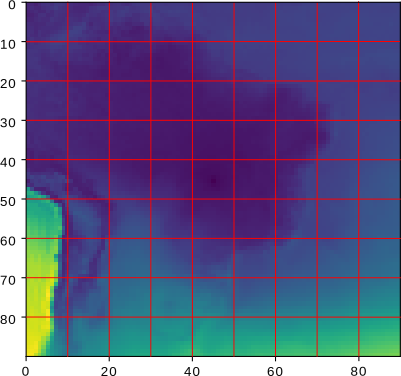
\includegraphics[scale=0.75]{../Figures/query_10x10_whole_real_brazil}
	\caption{Mesh to consider Spatio--Temporal Predictive Queries with Region of size $10 \times 10$.}
	\label{Fig:Query_10x10_whole_real_brazil}
\end{figure}

The results for $81$ spatio--temporal predictive queries, product of considering the mesh of squares ($10 \times 10$) over the domain, are described in the following table. For each domain partitioning scheme with $k = \left\{8, 66, 132 \right\}$, we present a descriptive statistics summary for the prediction query value computed. We can see the variation of mean and its respective standard deviation for the prediction value when considering the model composition formed by the representative models in each domain partitioning technique: $k$--Medoids and Regular.

\begin{table}[h!]
	\centering
	\tiny
	\begin{tabular}{|c|c|c|c|c|c|c|}
		\hline
		\multirow{2}{*}{Dom. Partitioning Technique} & \multicolumn{3}{c|}{$k$--Medoids} & \multicolumn{3}{c|}{Regular} \\
		\cline{2-7}
		& $k = 8$. & $k = 66$ & $k = 132$ & $k = 8$ & $k = 66$ & $k = 132$ \\
		\cline{2-7}
		\hline
		Forecast Error ($t_{f}=8$) & $0.48 \pm 0.59$ & $0.47 \pm 0.86$ & $0.39 \pm 0.62$ & $1.05 \pm 2.07$ & $1.17 \pm 2.59$ & $0.55 \pm 0.68$	 \\
%		Forecast Error ($t_{f}=8$) & $0.48 \pm 0.59$ & $0.47 \pm 0.86$ & $0.39 \pm 0.62$ & $1.05 \pm 2.07$ & $0.45 \pm 0.69$ & $0.44 \pm 0.66$	 \\
		\hline
	\end{tabular}
	\caption{Forecast Error Summary.}
	\label{Table:Query10x10_kMedoids_Regular_StatSummary}
\end{table}

According to Table \ref{Table:Query10x10_kMedoids_Regular_StatSummary}, the model composition formed by representative models of the $k$--Medoids representatives predict better than the regular approach. Analisis experimental que no es tan riguroso, pues solo muestra una variacion del error para regiones 
The following figures are heat maps of the computed forecast errors for the considered spatio--temporal predictive queries:

\begin{figure}[ht]
	\subfloat[$k$--Medoids.]{
		\begin{minipage}[c][1\width]{
				0.5\textwidth}
			\centering
			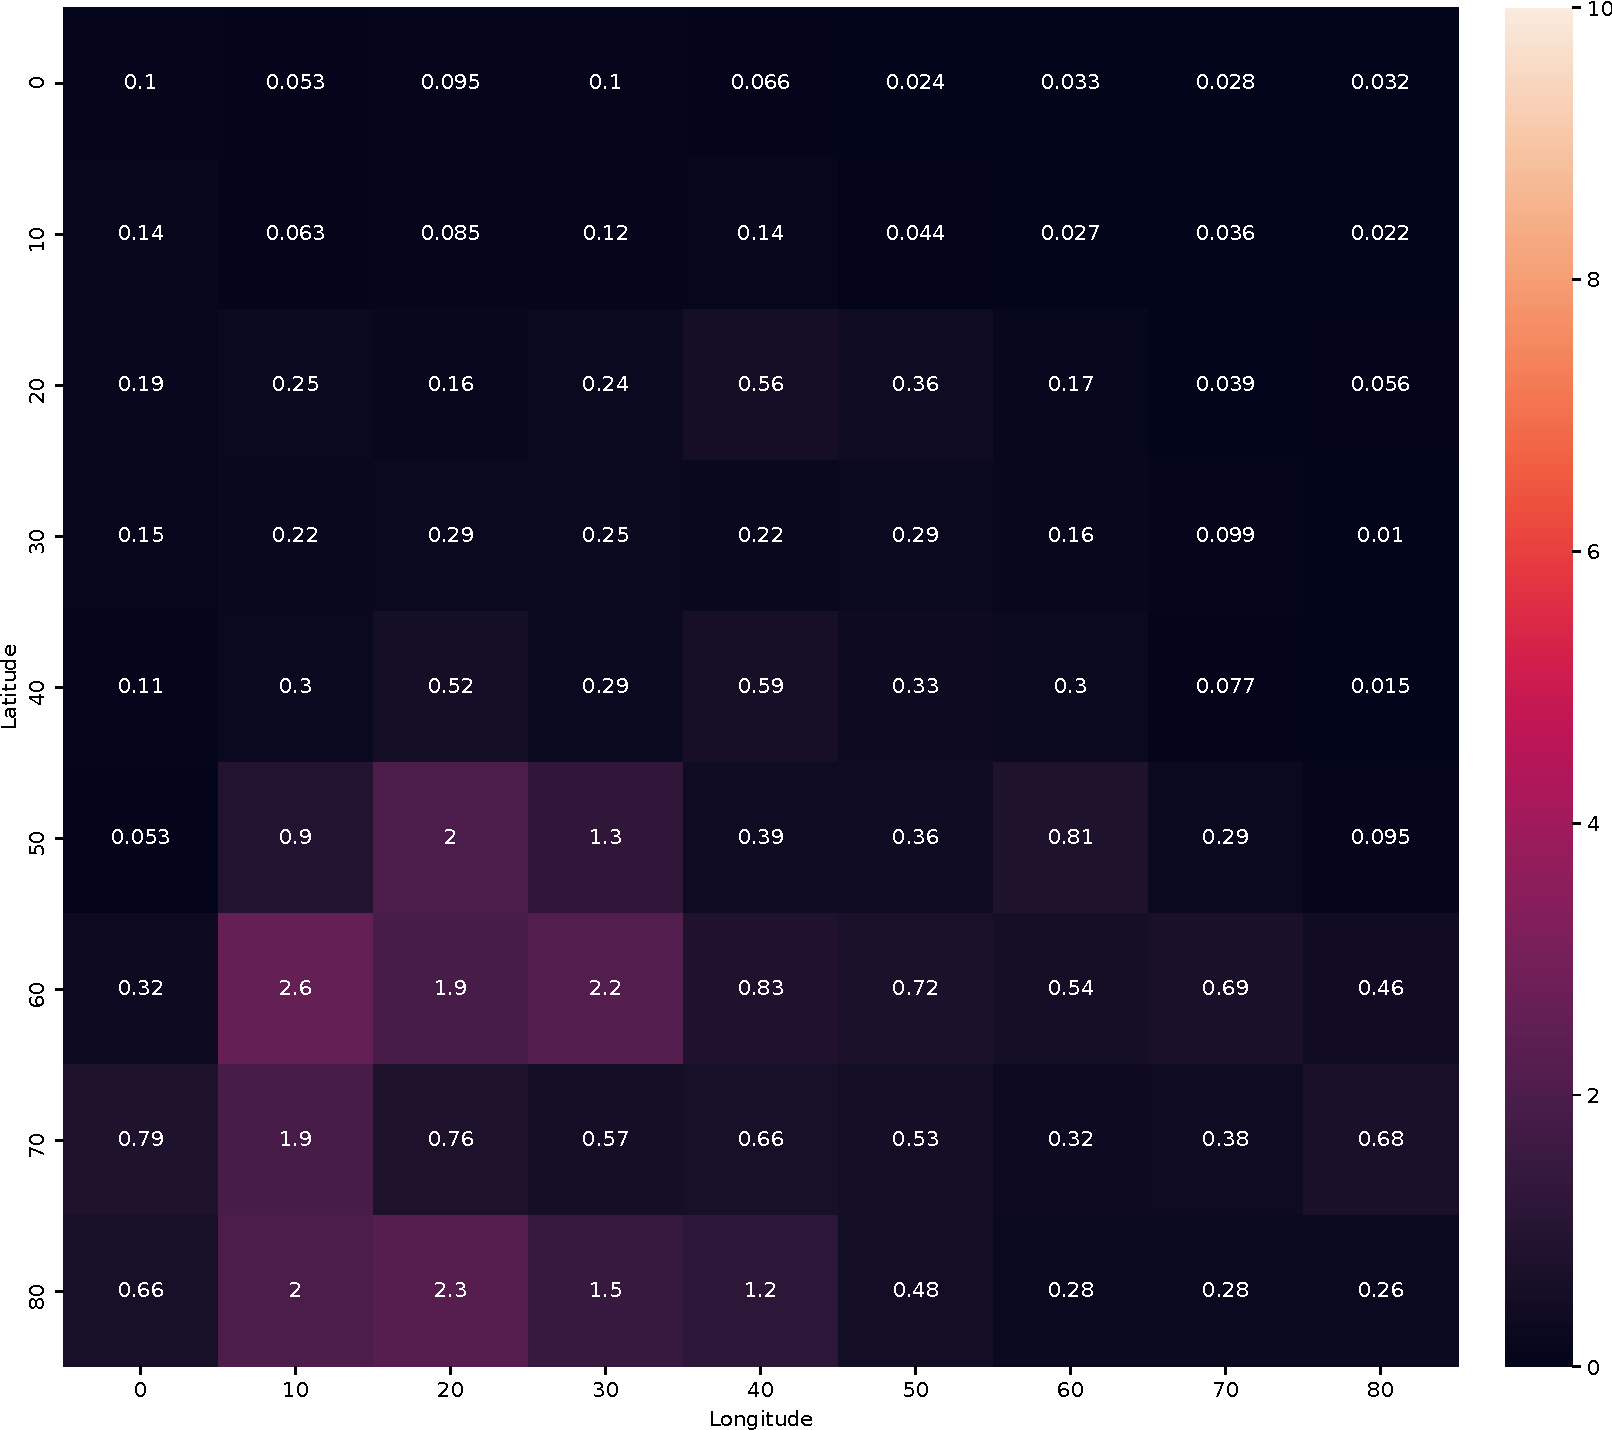
\includegraphics[width=1\textwidth]{../Figures/query_10x10_kmedoids_k8-300dpi}
	\end{minipage}}
	\hfill 	
	\subfloat[Regular.]{
		\begin{minipage}[c][1\width]{
				0.5\textwidth}
			\centering
			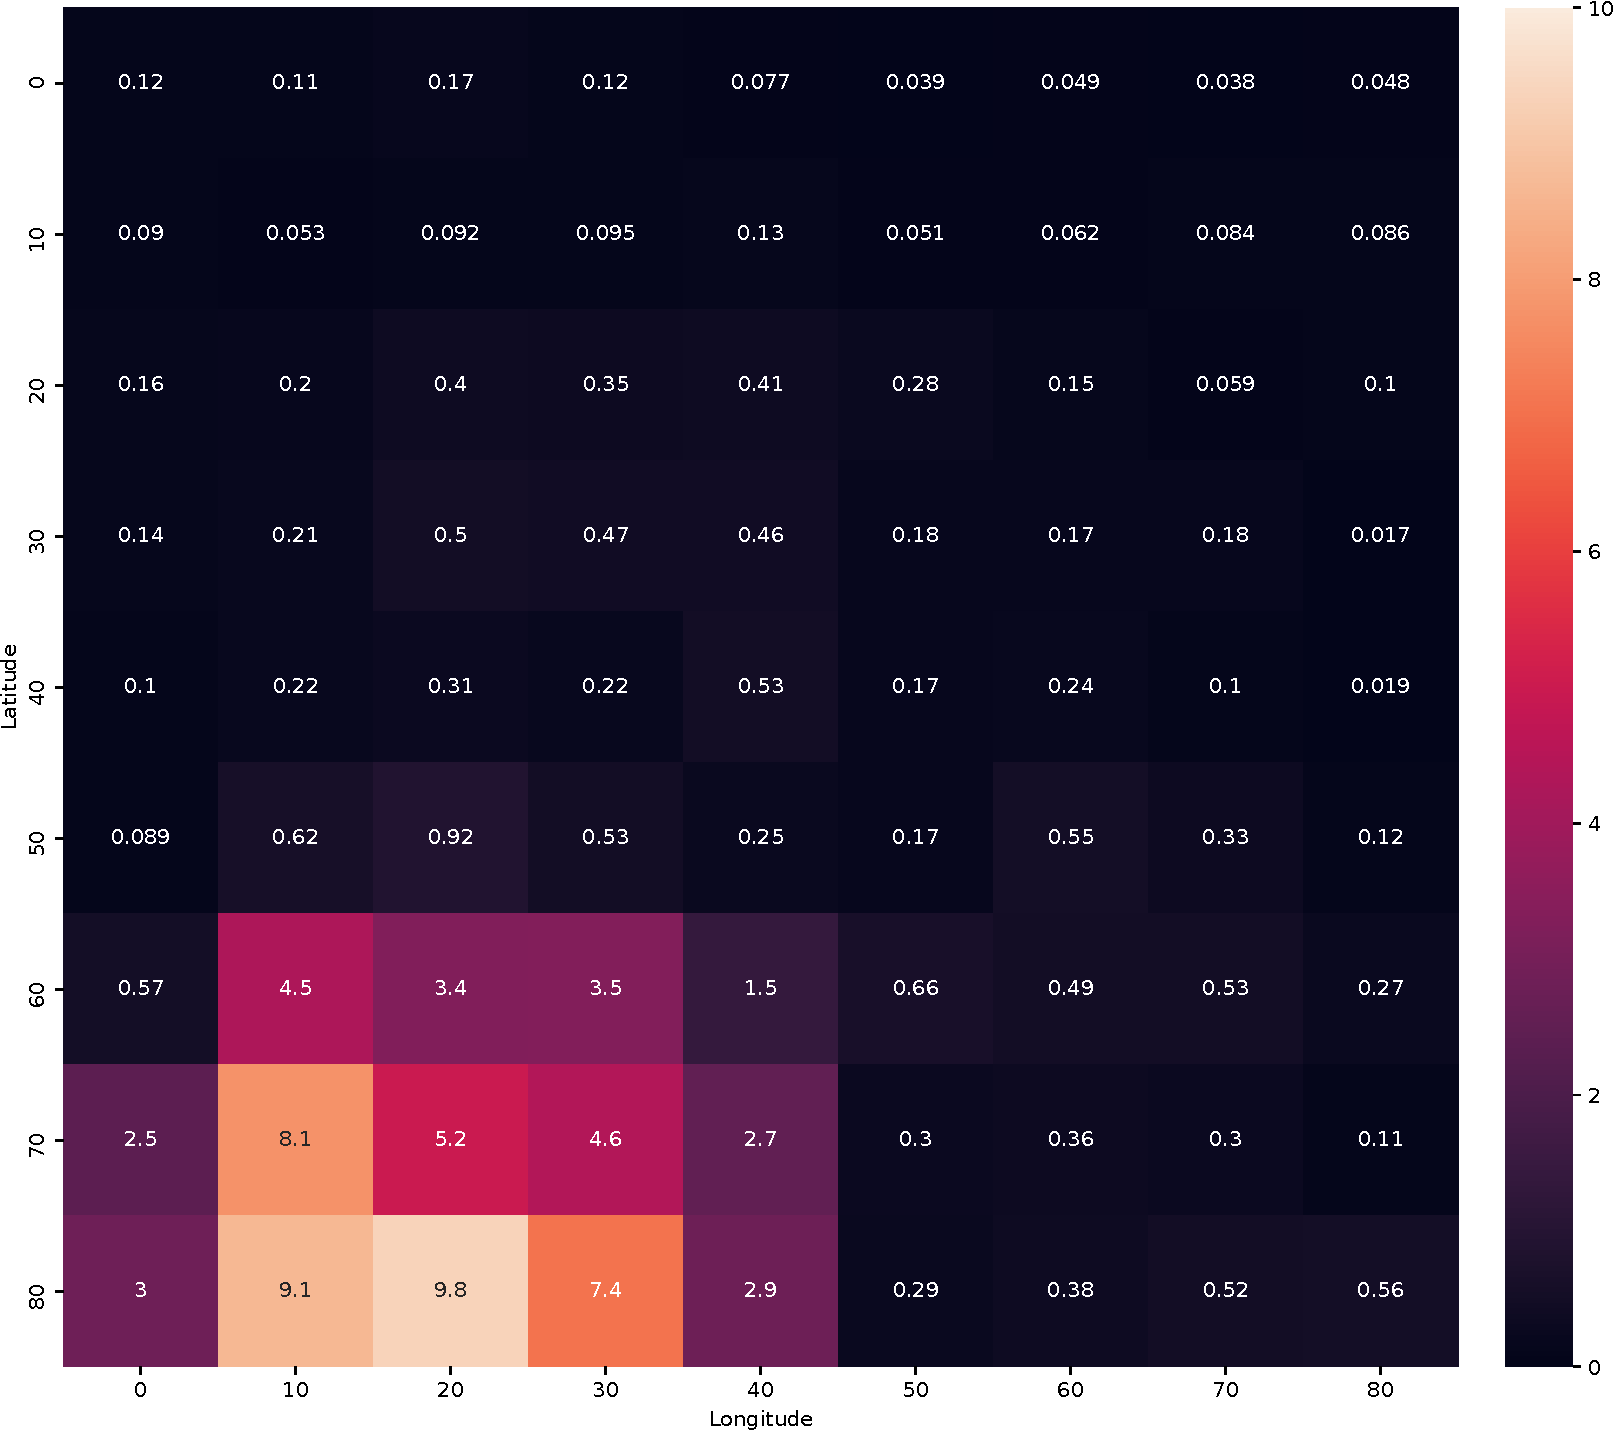
\includegraphics[width=1\textwidth]{../Figures/query_10x10_regular_k8-300dpi}
	\end{minipage}}
	\caption{Model Composition formed by Models Representatives in a Domain Partitioning Technique ($k=8$)}
	\label{Fig:query_10x10_kmedoids_regular_k8}
\end{figure}

\begin{figure}[h!]
	\subfloat[$k$--Medoids.]{
		\begin{minipage}[c][1\width]{
				0.5\textwidth}
			\centering
			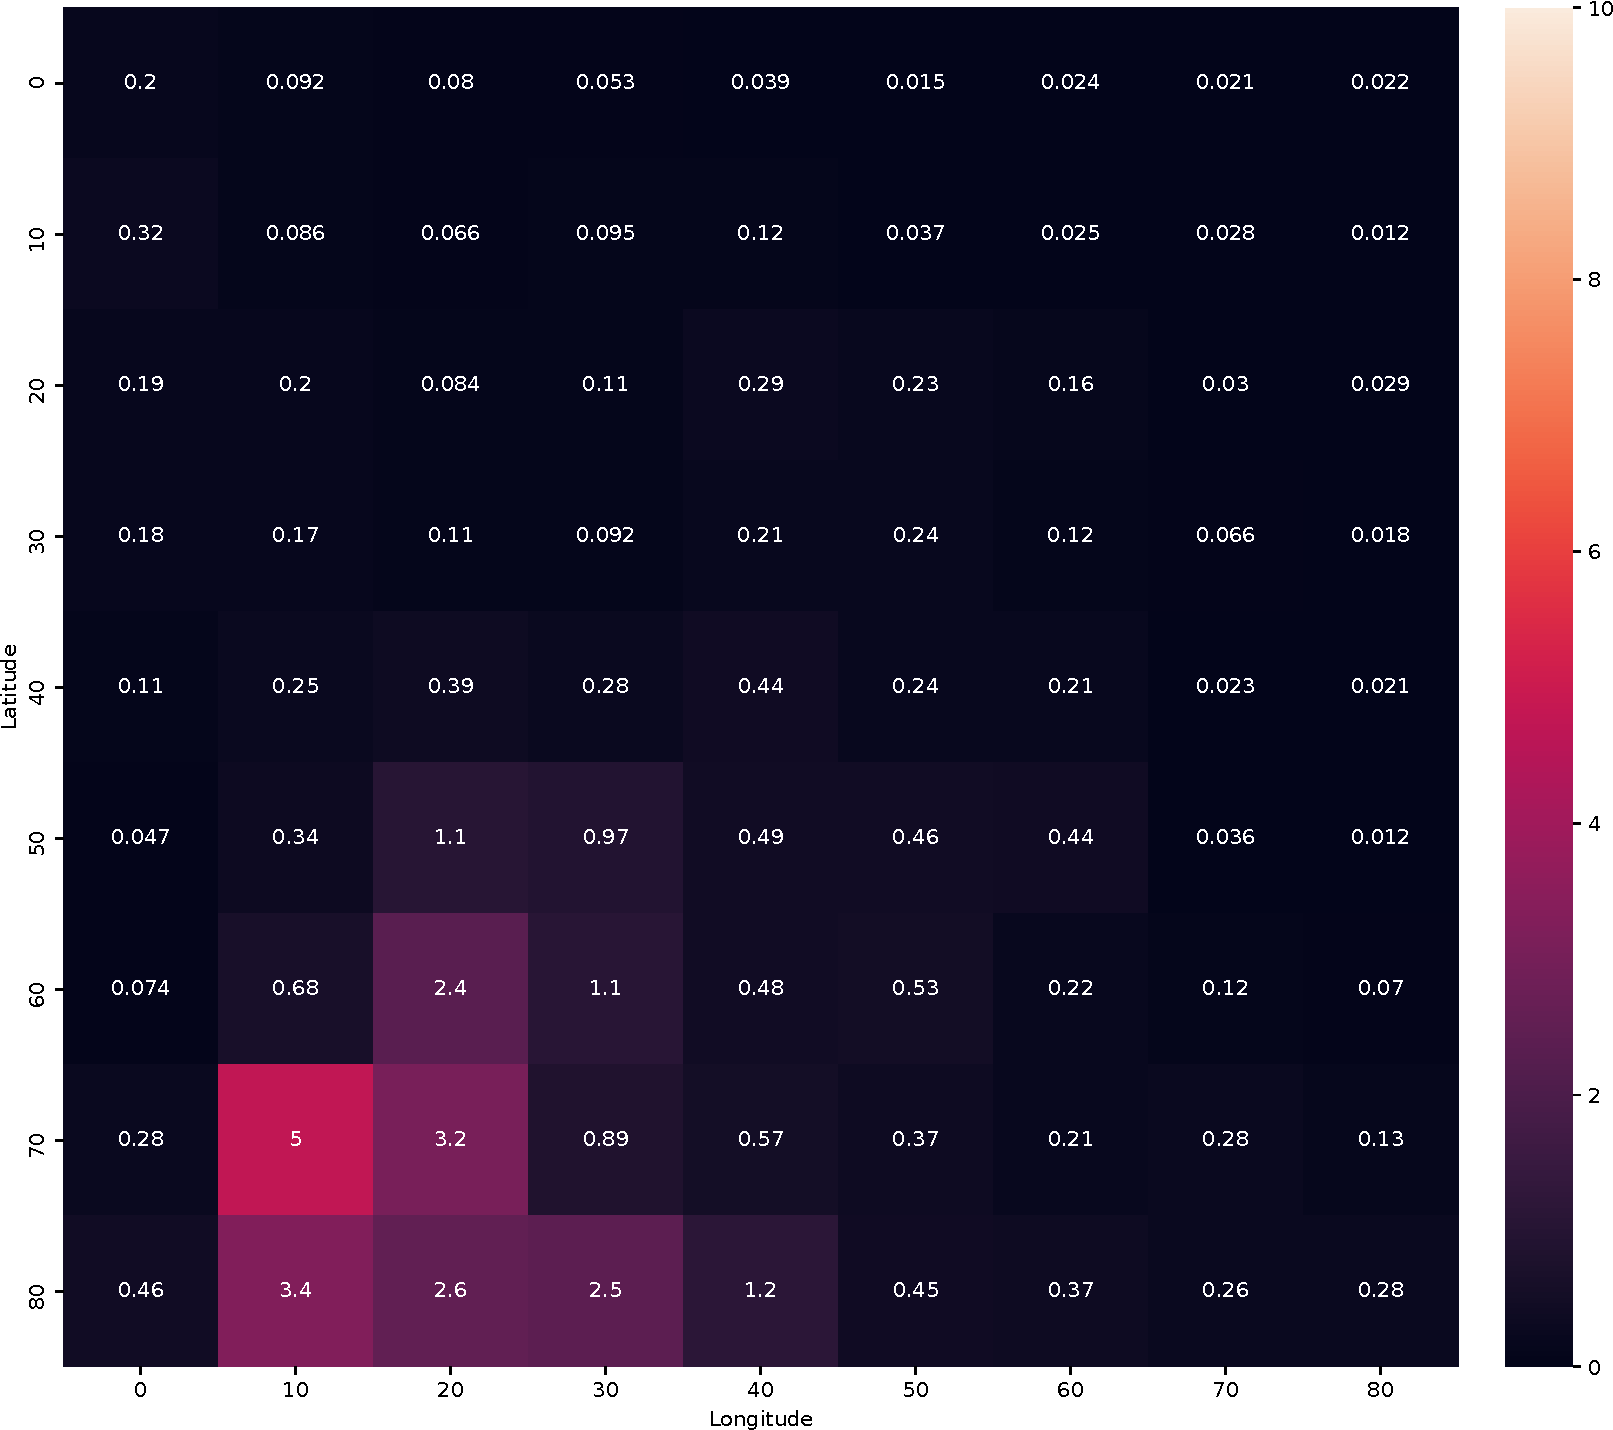
\includegraphics[width=1\textwidth]{../Figures/query_10x10_kmedoids_k66-300dpi}
	\end{minipage}}
	\hfill 	
	\subfloat[Regular.]{
		\begin{minipage}[c][1\width]{
				0.5\textwidth}
			\centering
			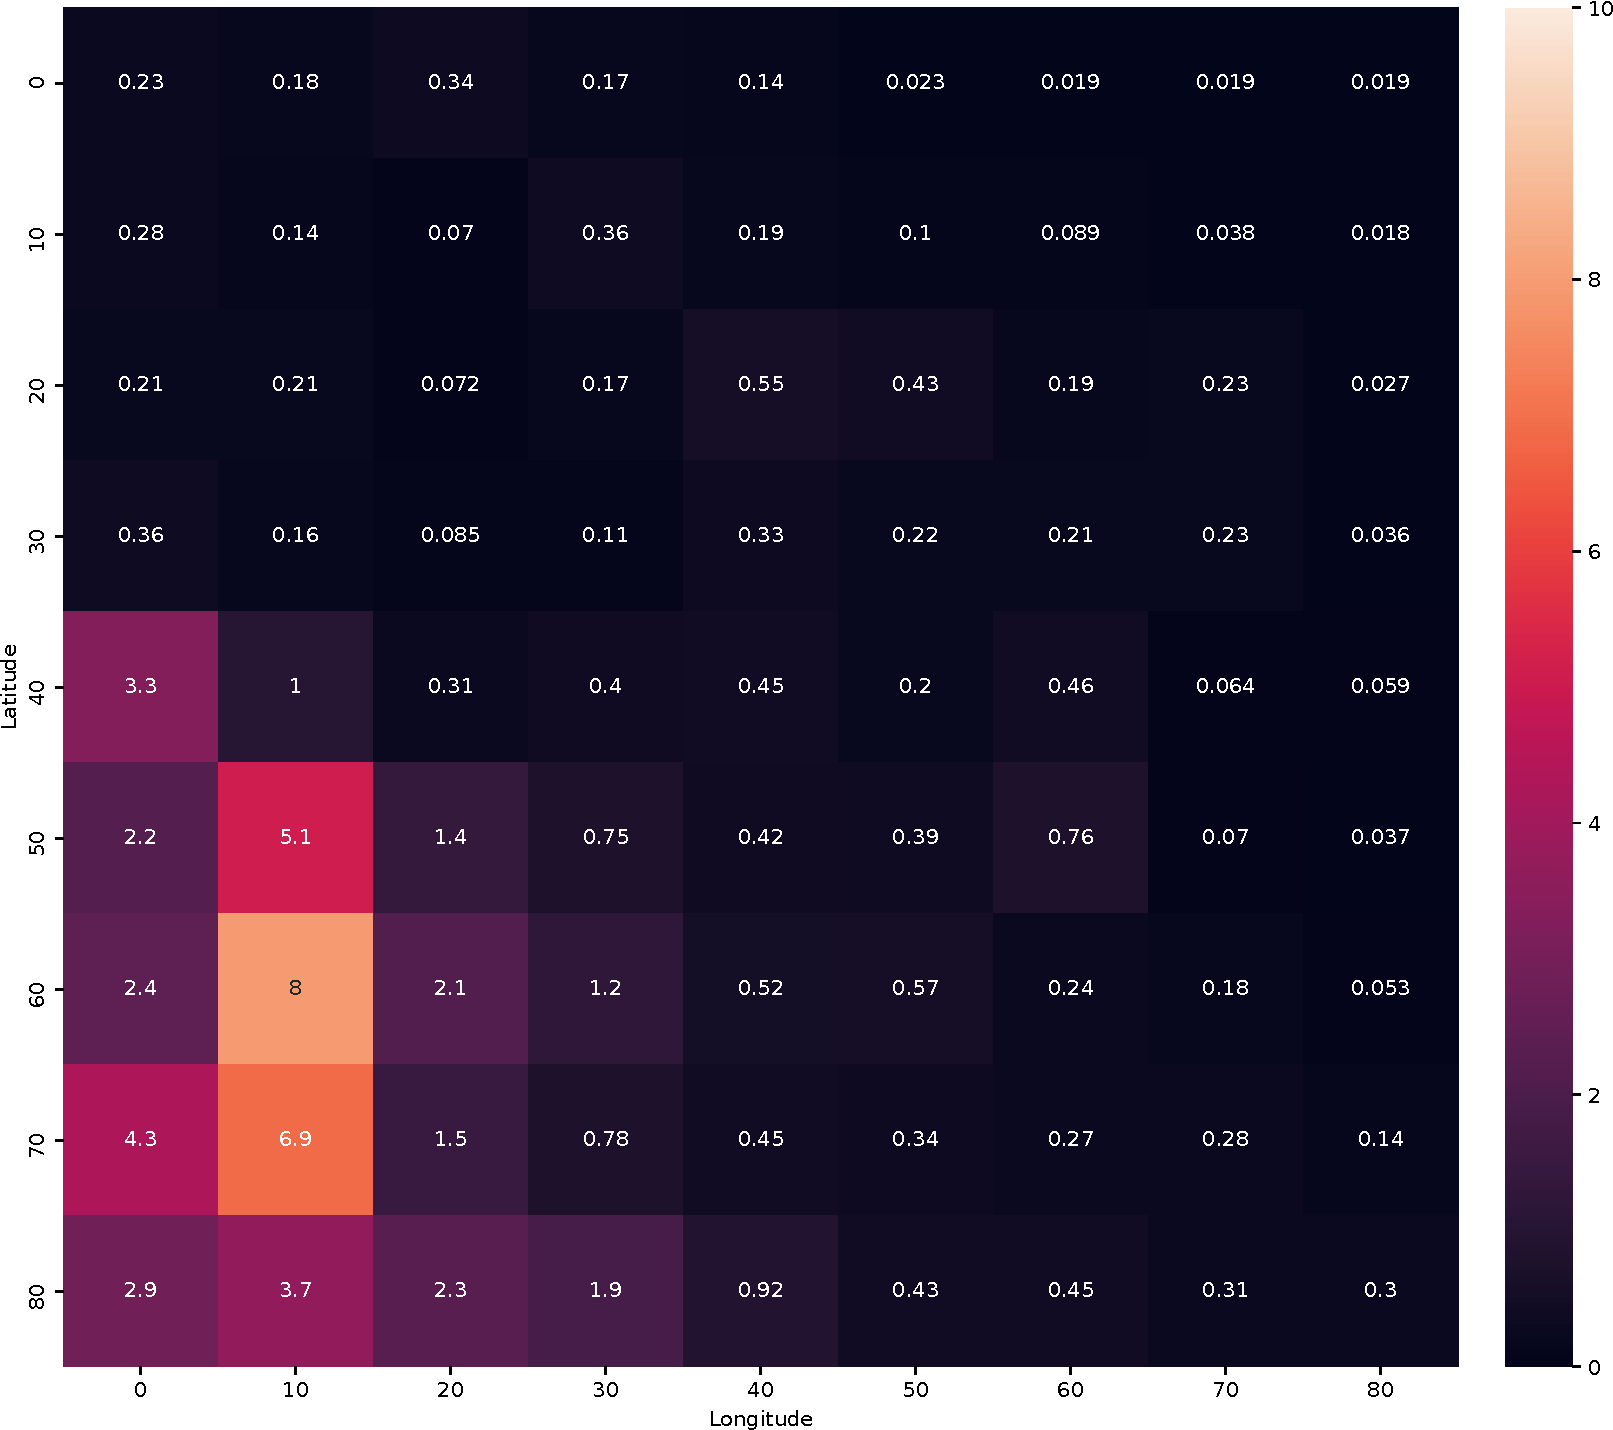
\includegraphics[width=1\textwidth]{../Figures/query_10x10_regular_k66_b-300dpi}
	\end{minipage}}
	\caption{Model Composition formed by Models Representatives in a Domain Partitioning Technique ($k=66$).}
	\label{Fig:query_10x10_kmedoids_regular_k66}
\end{figure}

\begin{figure}[h!]
	\subfloat[$k$--Medoids.]{
		\begin{minipage}[c][1\width]{
				0.5\textwidth}
			\centering
			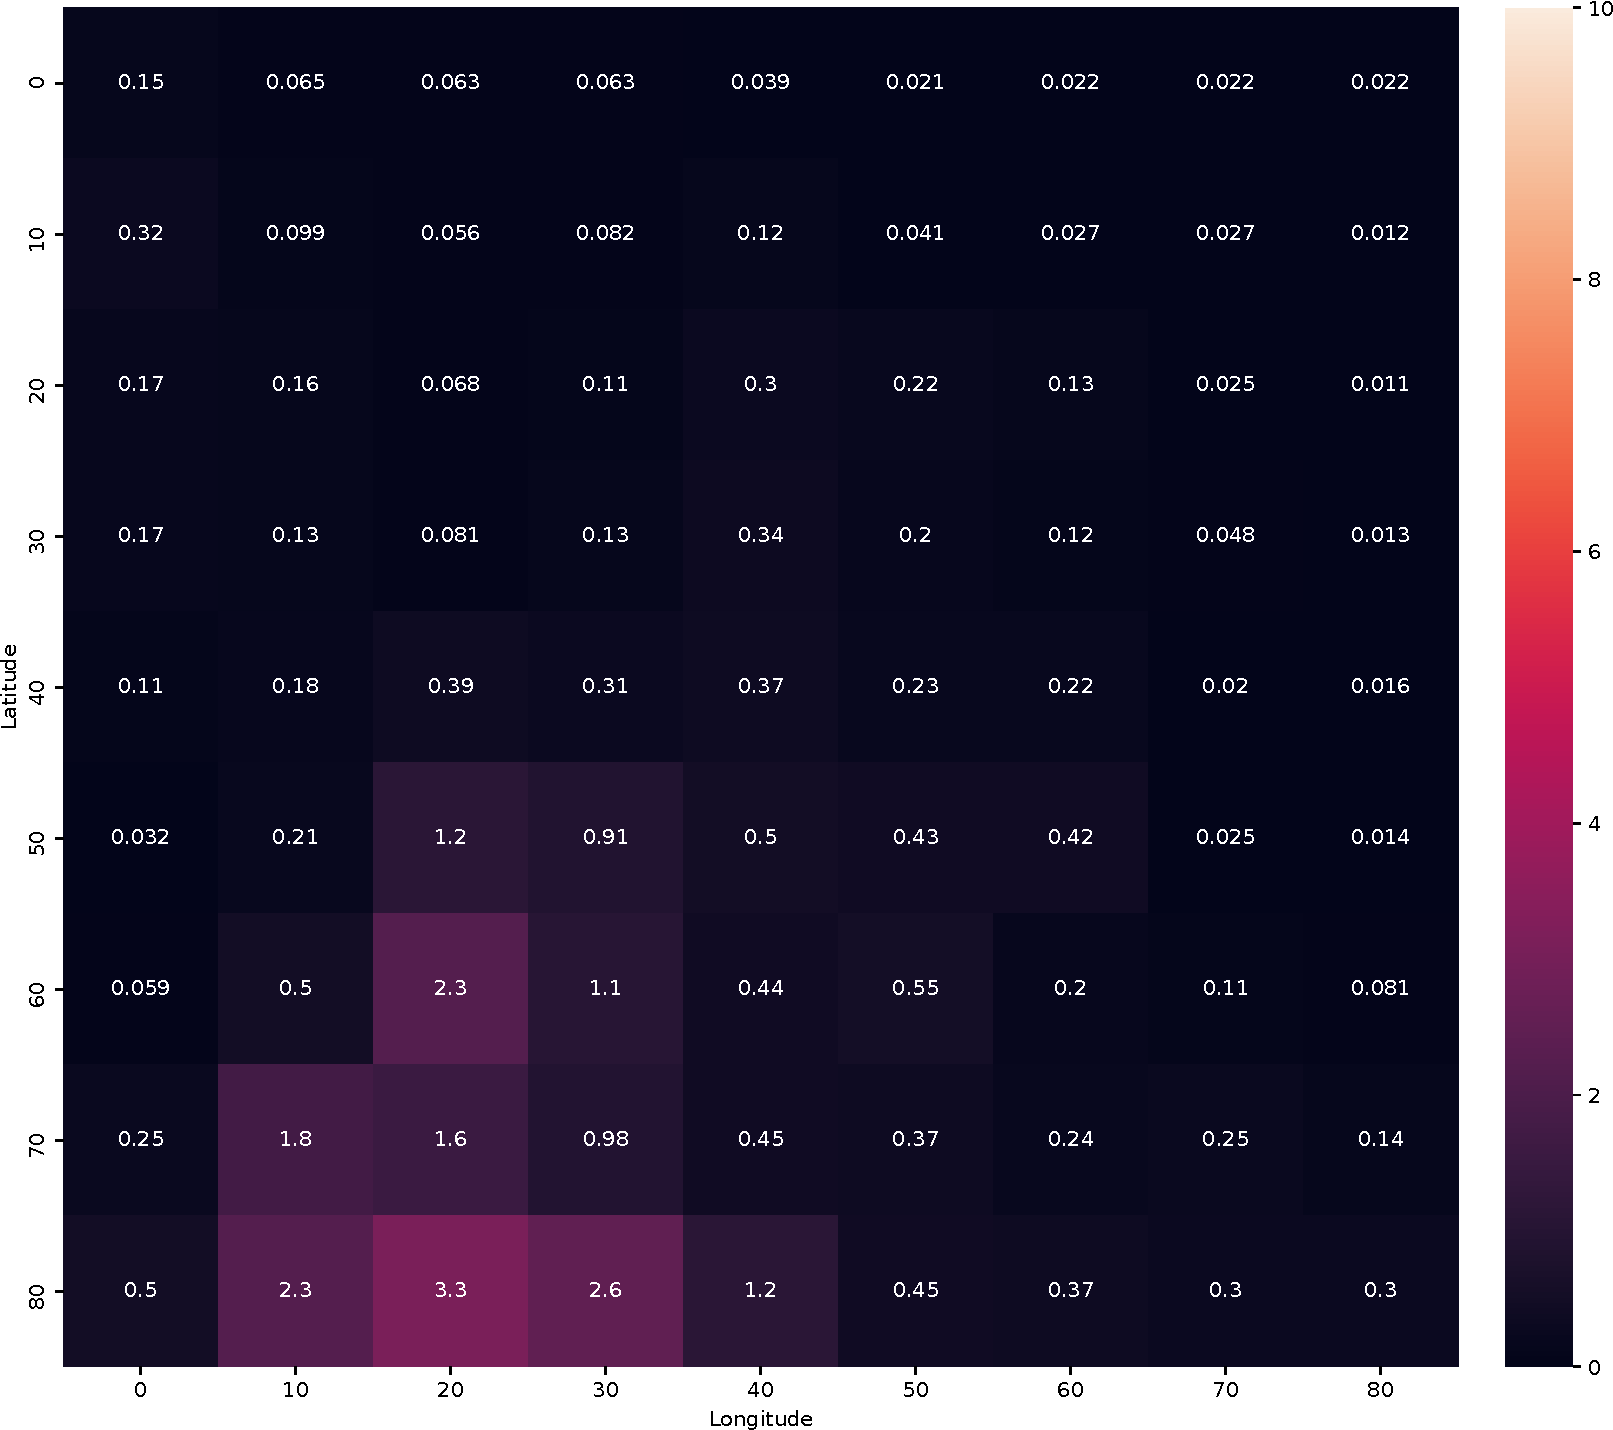
\includegraphics[width=1\textwidth]{../Figures/query_10x10_kmedoids_k132-300dpi}
	\end{minipage}}
	\hfill 	
	\subfloat[Regular.]{
		\begin{minipage}[c][1\width]{
				0.5\textwidth}
			\centering
			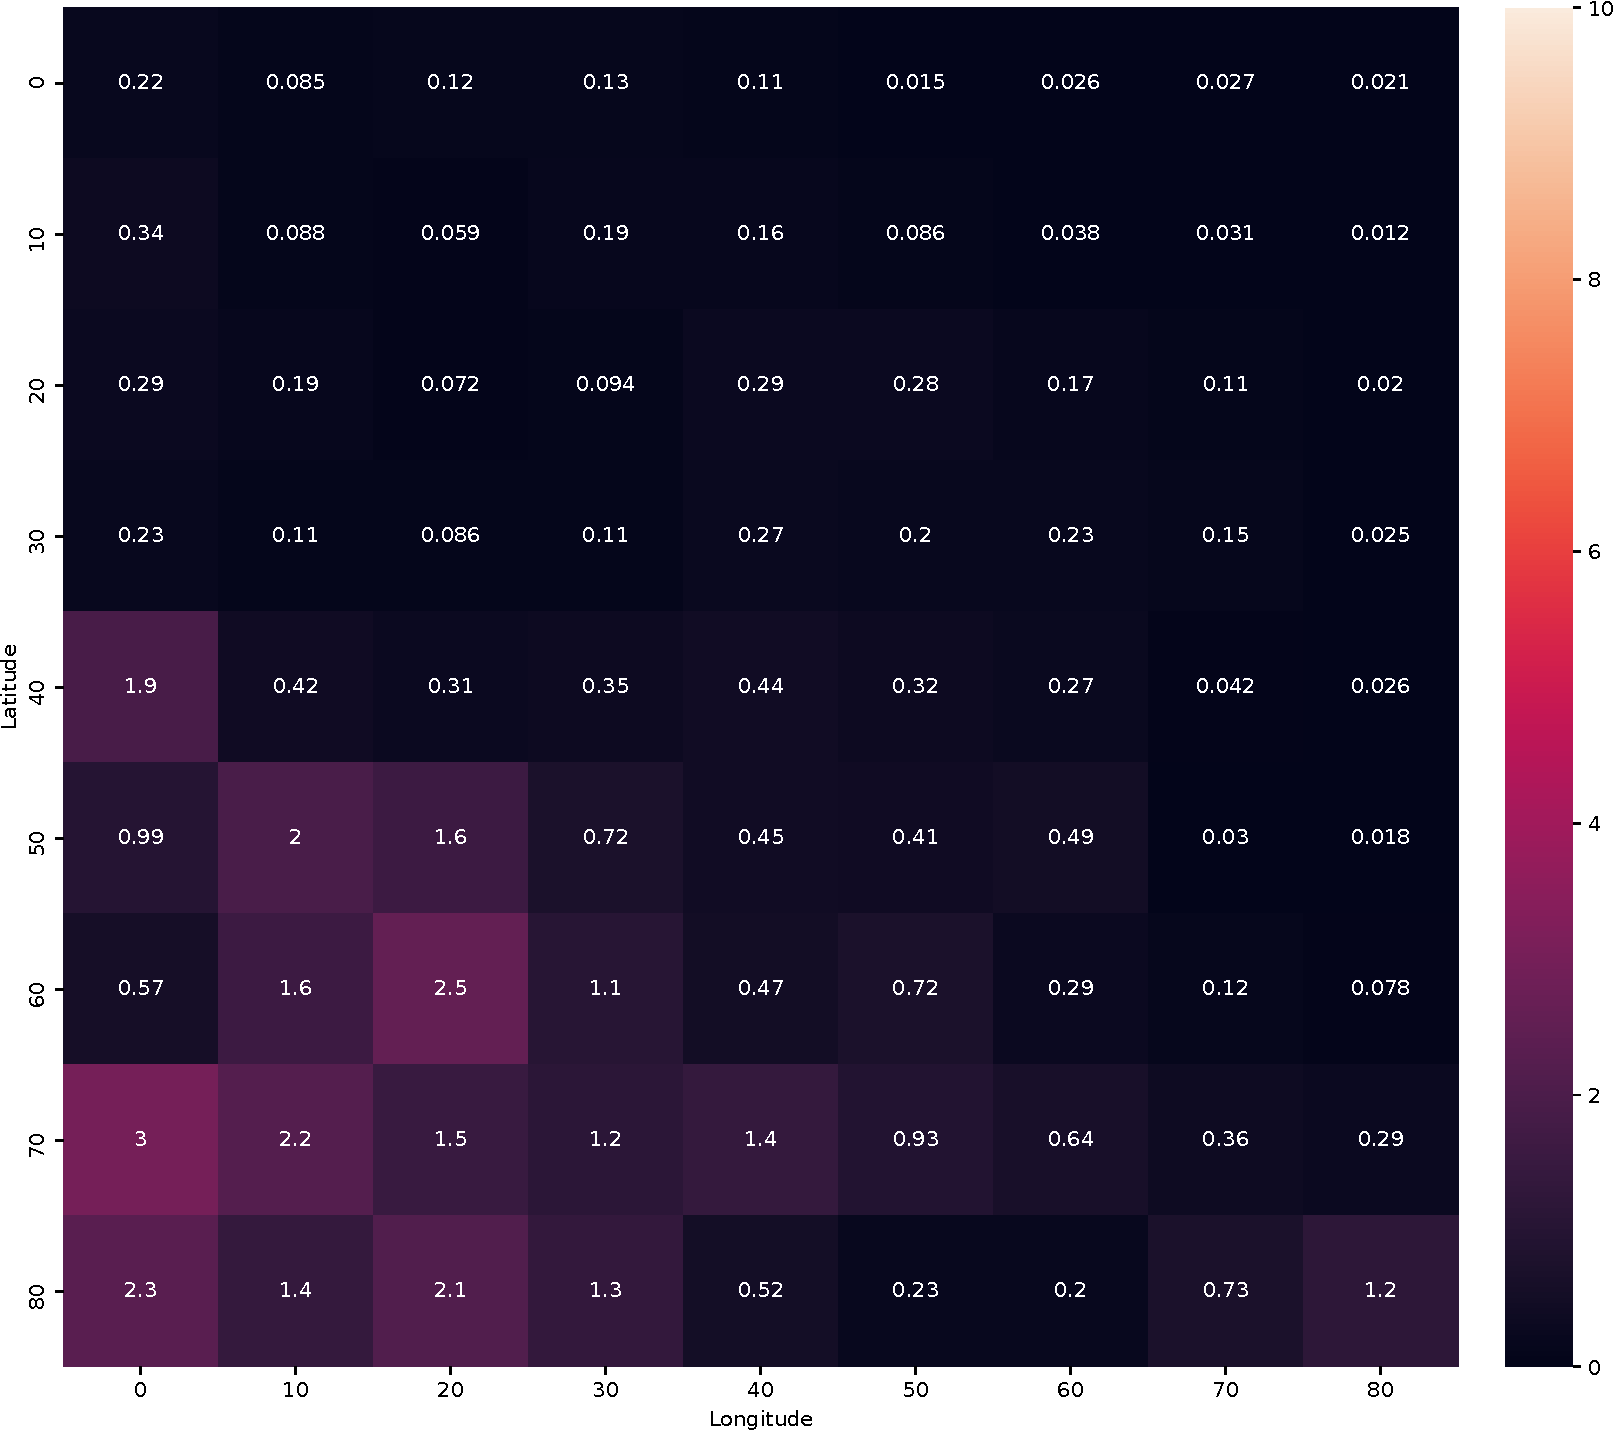
\includegraphics[width=1\textwidth]{../Figures/query_10x10_regular_k132_b-300dpi}
	\end{minipage}}
	\caption{Model Composition formed by Models Representatives in a Domain Partitioning Technique ($k=132$.)}
	\label{Fig:query_10x10_kmedoids_regular_k132}
\end{figure}

The experiments carried out in Sections \ref{Sec:AnalyzeDomainPartitioning} and \ref{Sec:AnalyzePredictorRepresentatives} enable the evaluation and analysis of the grouping quality for each partitioning technique, as well as the predictive quality of the models generated in the representative points, respectively. With these results we evaluate the predictive quality of the models generated in the representative points when they are used in the composition of models for the execution of a spatio-temporal predictive query. 
This representative generalizes the temporal evolution and its predictive model is within a prediction limit for future values.

Experimentally we observe that for different values of $k$, the composition of models also presents variations in the prediction values, this is due to the properties of spatio--temporal data. When we consider the presence of several domain partitioning schemes, we use the model classifier for time series, which corresponds to our proposal.

Next we show the results of model composition using the classifier of predictive models for univariate time--series, and also the results when the model composition is the point model generation.

\begin{table}[h!]
	\centering
	\tiny
	\begin{tabular}{|c|c|c|}
		\hline
		Model Composition & Model Classifier & Model Each Point (ARIMA)\\
		\hline
		Forecast Error ($t_{f}=8$) & $1.07 \pm 1.59$ & $0.38 \pm 0.61$ \\
		\hline
	\end{tabular}
	\caption{Forecast Error Summary.}
	\label{Table:Query10x10_Classfier_Point_Each_StatSummary}
\end{table}
In the following Figure we show the heat map for the prediction values computed during the query execution.

\begin{figure}[h!]
	\subfloat[$k$--Medoids.]{
		\begin{minipage}[c][1\width]{
				0.5\textwidth}
			\centering
			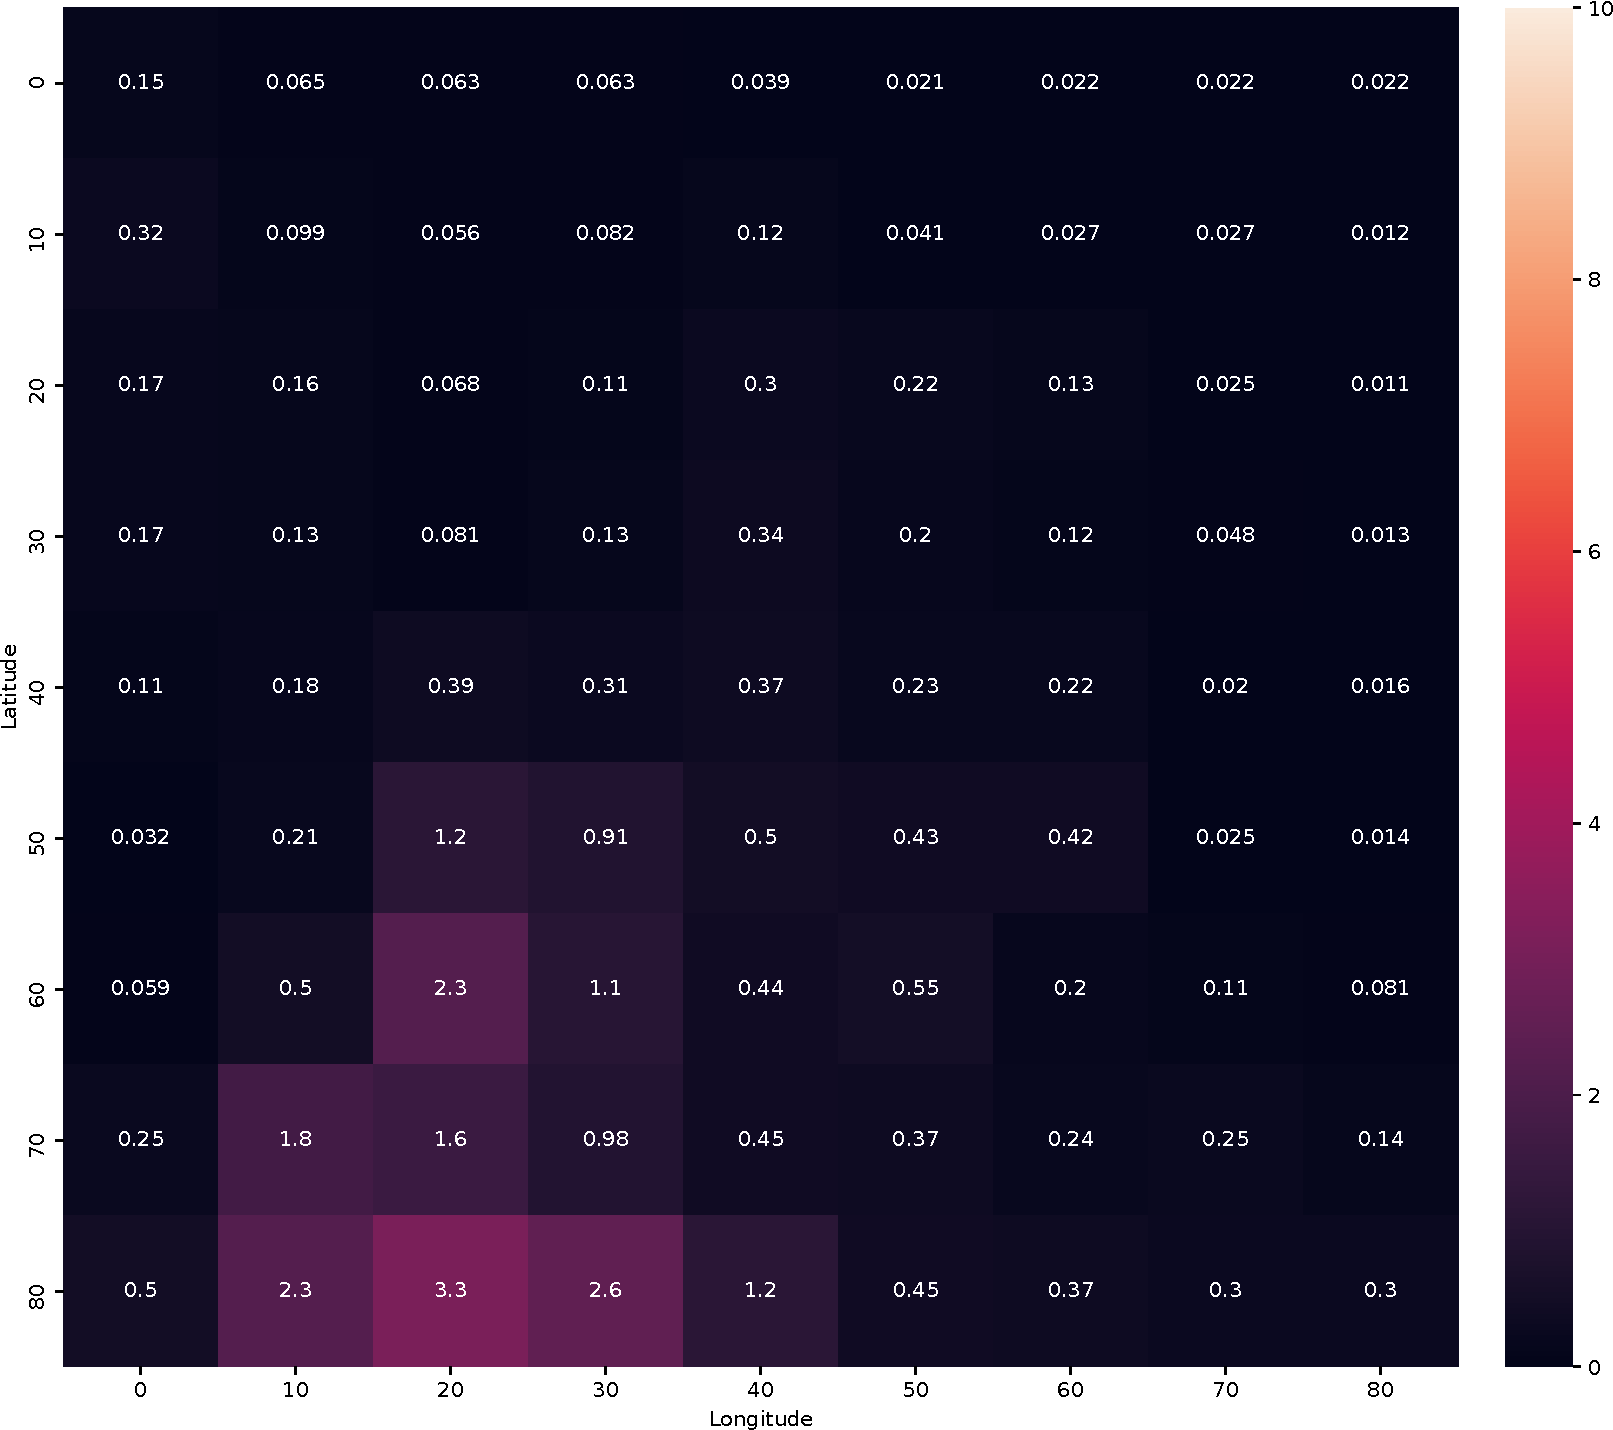
\includegraphics[width=1\textwidth]{../Figures/query_10x10_kmedoids_k132-300dpi}
	\end{minipage}}
	\hfill 	
	\subfloat[Regular.]{
		\begin{minipage}[c][1\width]{
				0.5\textwidth}
			\centering
			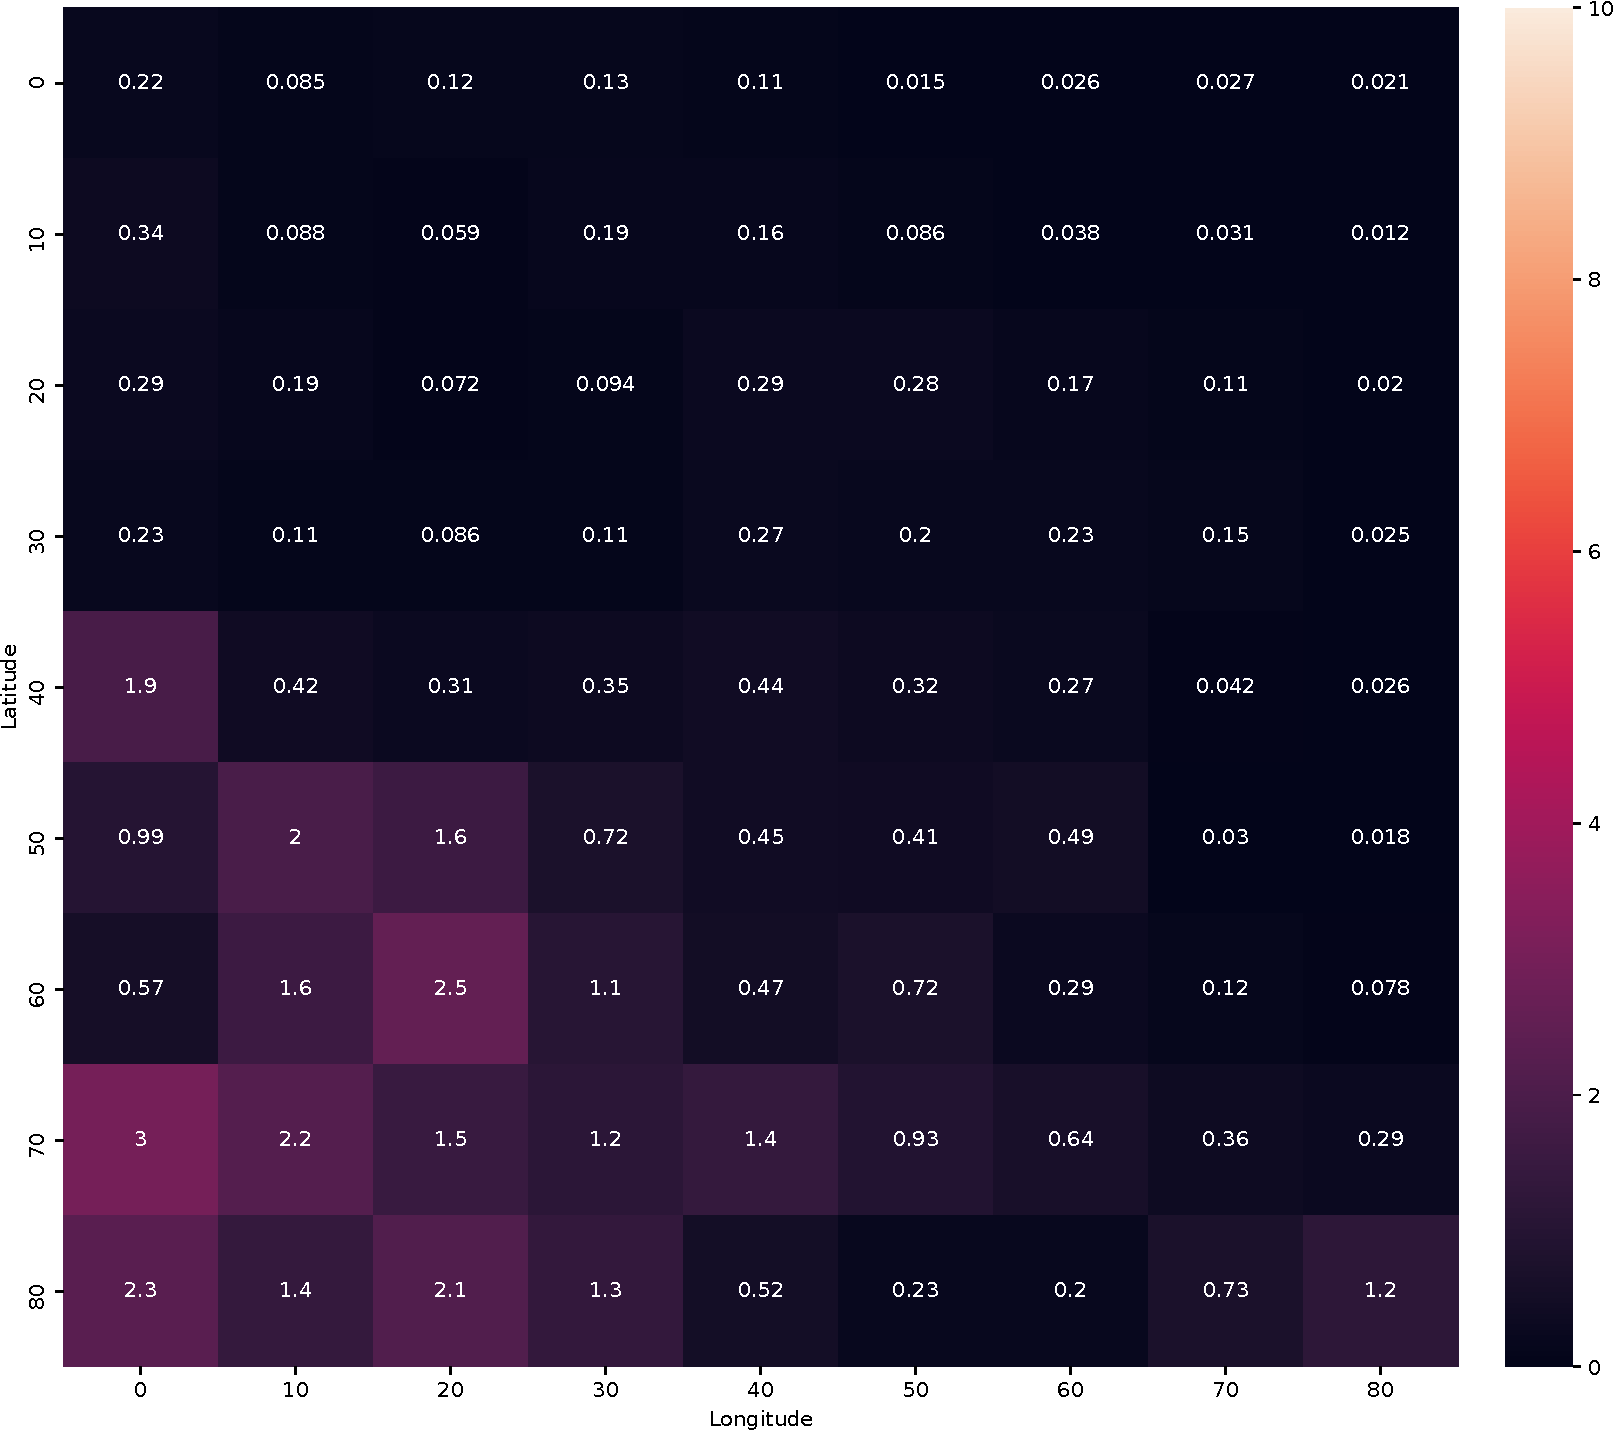
\includegraphics[width=1\textwidth]{../Figures/query_10x10_regular_k132_b-300dpi}
	\end{minipage}}
	\caption{Model Composition by Models Representatives in a Domain Partitioning Technique ($k=132$.)}
	\label{Fig:query_10x10_classifier_each}
\end{figure}

The next table shows the region size and the total number of queries considered to compute its predictions:

\begin{table}[h]	\centering
	\tiny
	\begin{tabular}{|c|c|r|r|r|r|r|r|r|r|r|}
		\hline
		\multirow{3}{*}{Size} & \multirow{3}{*}{Query Region} & \multicolumn{9}{c|}{Model Composition} \\ 
		\cline{3-11}
		& & \multicolumn{3}{c|}{$k$--Medoids} & \multicolumn{3}{c|}{Regular} & \multirow{2}{*}{Classifier} & \multirow{2}{*}{$k$NN} & \multirow{2}{*}{ARIMA} \\ 
		\cline{3-8}
		& & $k =8$ & $k = 66$ & $k = 132$ & $k=8$  & $k = 66$ & $k = 132$ &  & & \\ \hline % & DJEnsemble \\ \hline
		$20 \times 20$ & $[ 0, 20] \times [ 0, 20]$ & 0.089 & 0.174 & 0.160 & 0.094 & 0.169 & 0.205 & 0.190 & 0.209 & 0.158  \\ % &  935.748\\ %30.590 \\
		$20 \times 20$ & $[20, 40] \times [35, 55]$ & 0.335 & 0.199 & 0.230 & 0.395 & 0.234 & 0.225 & 0.330 & 0.258 & 0.203 \\ % &  993.826\\ %31.525 \\
		$20 \times 20$ & $[50, 70] \times [60, 80]$ & 0.584 & 0.203 & 0.188 & 0.475 & 0.165 & 0.186 & 0.274 & 0.145 & 0.170 \\ % & 6572.021\\ %81.068 \\
		$20 \times 20$ & $[15, 35] \times [65, 85]$ & 0.063 & 0.045 & 0.038 & 0.106 & 0.074 & 0.057 & 0.093 & 0.067 & 0.034 \\ % & 4641.424\\%68.128 \\
		$30 \times 30$ & $[20, 50] \times [50, 80]$ & 0.203 & 0.147 & 0.135 & 0.170 & 0.180 & 0.158 & 0.202 & 0.210 & 0.122 \\ % & 1410.378\\%37.555 \\
		$30 \times 30$ & $[15, 45] \times [20, 50]$ & 0.262 & 0.155 & 0.168 & 0.367 & 0.199 & 0.184 & 0.281 & 0.198 & 0.156 \\ %  & 1205.687\\%34.723 \\
		$15 \times 20$ & $[40, 55] \times [20, 40]$ & 0.707 & 0.530 & 0.541 & 0.368 & 0.682 & 0.581 & 0.618 & 0.707 & 0.483 \\ % &  905.829\\%30.097 \\
		$15 \times 20$ & $[65, 80] \times [50, 70]$ & 0.470 & 0.302 & 0.308 & 0.353 & 0.266 & 0.300 & 0.343 & 0.190 & 0.248\\ %& 6382.732\\%79.892 \\
		$30 \times 15$ & $[30, 60] \times [ 5, 20]$ & 0.353 & 0.205 & 0.147 & 0.273 & 0.318 & 0.293 & 0.391 & 0.208 & 0.137 \\ % &  950.797\\%30.835 \\
		$30 \times 15$ & $[10, 40] \times [55, 70]$ & 0.139 & 0.111 & 0.098 & 0.127 & 0.158 & 0.115 & 0.135 & 0.226 & 0.095 \\ %& 4546.940\\ \hline% 67.431 \\ 
		\hline
	\end{tabular}
	\caption{MSE Forecast Error for Spatio-Temporal Queries in the domain $\mathcal{D}$.}
	\label{Table:MSEForecasError}
\end{table}

The latitude and longitude for the queries are:

%Query size 20 x 20
%Uno
%Lat : (7.5) - (-2.5) 
%Long: (285.5) - (295.5)
%
%Dos
%Lat : (7.5) - (-12.5)
%Lon : (285.5) - (295.5)
%
%Tres (Cobre RJ)
%Lat : (-17.5) - (-27.5)
%Lon : (315.5) - (325.5)
%
%Cuatro
%Lat : (0) - (-10)
%Lon : 318 - 328
%
%Query Size 30 x 30
%Cinco
%Lat : (-2.5) - (-17.5)
%Lon : (310.5) - (325.5)
%
%Seis
%Lat : (0) - (-15)
%Lon : (295.5) - (310.5)
%
%Query Size 15 x 20
%Siete
%Lat : (-12.5) - (-20)
%Lon : (295.5) - (305.5)
%
%Ocho
%Lat : (-25) - (-32.5)
%Lon : (316.5) - (326.5) 
%
%Query Size 30 x 15
%Nueve 
%Lat : (-7.5) - (-22.5)
%Lon : (288) - (295.5) 
%
%Diez
%Lat : (2.5) - (-12.5)
%Lon : (319) - (326.5)

\section{Results and Discussion} 

The first part of this Chapter we describe the SPTA-TSA, an application developed to implement and analyze the proposed methodology. Next, we describe the outline of experiments and analysis performed to validate our hypothesis and decisions. 



\section{Final Comments}
